\def\allfiles{}%允许单文件编译
%生成目录超链接，使用UTF8字符集
\documentclass[12pt,UTF8]{ctexart}


\usepackage{mathtools}%花括号括起的公式
\usepackage{enumerate}%列表
\usepackage{graphicx}%表格
\usepackage[table]{xcolor}%彩色表格
\usepackage{booktabs}%调整表格行高


\renewcommand\tabcolsep{50pt}
\renewcommand\arraystretch{2}

%文本框
\usepackage{tcolorbox}
\tcbuselibrary{skins,vignette,raster,listings,listingsutf8,theorems, breakable,magazine,fitting}

%页面设置
\usepackage{geometry}%设置页面
\usepackage{setspace}%设置局部行距

\usepackage{ctex}
\usepackage{CJK}

%图像处理
\usepackage{graphicx}
\usepackage{float}%允许浮动
\usepackage{caption}%设置标题
\usepackage{graphicx, subfig}

%附录
\usepackage[toc,page]{appendix}

%导言区
\title{中小微企业的信贷决策}

%不要页眉
\pagestyle{plain}
\bibliographystyle{plain}

\geometry{a4paper}%将纸张设置为A4大小

%修改文档结构层次的名称
\usepackage{titlesec}%chapter1修改为一
\titleformat{\part}{\centering\Huge\bfseries}{\thepart}{1em}{}
\renewcommand\thepart{\chinese{part}}

%subsubsubsection的使用
%\usepackage{titlesec}
%\titleclass{\subsubsubsection}{straight}[\subsection]
%
%\newcounter{subsubsubsection}[subsubsection]
%\renewcommand\thesubsubsubsection{\thesubsubsection.\arabic{subsubsubsection}}
%\renewcommand\theparagraph{\thesubsubsubsection.\arabic{paragraph}}
%
%\titleformat{\subsubsubsection}
%{\normalfont\normalsize\bfseries}{\thesubsubsubsection}{1em}{}
%\titlespacing*{\subsubsubsection}
%{0pt}{3.25ex plus 1ex minus .2ex}{1.5ex plus .2ex}
%
%\makeatletter
%\renewcommand\paragraph{\@startsection{paragraph}{5}{\z@}%
%	{3.25ex \@plus1ex \@minus.2ex}%
%	{-1em}%
%	{\normalfont\normalsize\bfseries}}
%\renewcommand\subparagraph{\@startsection{subparagraph}{6}{\parindent}%
%	{3.25ex \@plus1ex \@minus .2ex}%
%	{-1em}%
%	{\normalfont\normalsize\bfseries}}
%\def\toclevel@subsubsubsection{4}
%\def\toclevel@paragraph{5}
%\def\toclevel@paragraph{6}
%\def\l@subsubsubsection{\@dottedtocline{4}{7em}{4em}}
%\def\l@paragraph{\@dottedtocline{5}{10em}{5em}}
%\def\l@subparagraph{\@dottedtocline{6}{14em}{6em}}
%\makeatother
%
%\setcounter{secnumdepth}{4}
%前缀
%主文件开始


\begin{document}

{\kaishu
%处理封面
% Remove the author and date fields and the space associated with them
% from the definition of maketitle!
\makeatletter
\renewcommand{\@maketitle}{
	\newpage
	\null
	\vskip 2em%
	\begin{center}%
		{\LARGE \@title \par}%
	\end{center}%
	\par} \makeatother

\maketitle




%This template Powered by Ruiyang Zhou.
%！警告！
%提交修改时务必删去或忽略掉LaTeX编译所产生的其他文件，避免推送和拉取时出现冲突！

%说明1
%先编译主文档，然后再修改和编译分文档时会自动出现完整内容，无需再次编译主文档。这里是利用了TexStuio自动识别主文档的机制。
%说明2
%在TexStuio中的选项-主文档设置-将当前文档设置为主文档，可以只编译该分文档。此法适用于主文档因内容过多而编译时间过长的时候。
%说明3
%TeX文件的命名由三部分组成：编号_英文名[序号]
%编号中，00单列；0是摘要；1，2，3……代表该文件在论文中的次序


%Part1:TeX文件
%00_MASTER是主文档，管理封面，并汇总分文件的代码输出LaTeX结果
%00_prefix是各个文档的前缀，负责管理package和导言区
%00_template是分文件模板

\ifx\allfiles\undefined
%生成目录超链接，使用UTF8字符集
\documentclass[12pt,UTF8]{ctexart}


\usepackage{mathtools}%花括号括起的公式
\usepackage{enumerate}%列表
\usepackage{graphicx}%表格
\usepackage[table]{xcolor}%彩色表格
\usepackage{booktabs}%调整表格行高


\renewcommand\tabcolsep{50pt}
\renewcommand\arraystretch{2}

%文本框
\usepackage{tcolorbox}
\tcbuselibrary{skins,vignette,raster,listings,listingsutf8,theorems, breakable,magazine,fitting}

%页面设置
\usepackage{geometry}%设置页面
\usepackage{setspace}%设置局部行距

\usepackage{ctex}
\usepackage{CJK}

%图像处理
\usepackage{graphicx}
\usepackage{float}%允许浮动
\usepackage{caption}%设置标题
\usepackage{graphicx, subfig}

%附录
\usepackage[toc,page]{appendix}

%导言区
\title{中小微企业的信贷决策}

%不要页眉
\pagestyle{plain}
\bibliographystyle{plain}

\geometry{a4paper}%将纸张设置为A4大小

%修改文档结构层次的名称
\usepackage{titlesec}%chapter1修改为一
\titleformat{\part}{\centering\Huge\bfseries}{\thepart}{1em}{}
\renewcommand\thepart{\chinese{part}}

%subsubsubsection的使用
%\usepackage{titlesec}
%\titleclass{\subsubsubsection}{straight}[\subsection]
%
%\newcounter{subsubsubsection}[subsubsection]
%\renewcommand\thesubsubsubsection{\thesubsubsection.\arabic{subsubsubsection}}
%\renewcommand\theparagraph{\thesubsubsubsection.\arabic{paragraph}}
%
%\titleformat{\subsubsubsection}
%{\normalfont\normalsize\bfseries}{\thesubsubsubsection}{1em}{}
%\titlespacing*{\subsubsubsection}
%{0pt}{3.25ex plus 1ex minus .2ex}{1.5ex plus .2ex}
%
%\makeatletter
%\renewcommand\paragraph{\@startsection{paragraph}{5}{\z@}%
%	{3.25ex \@plus1ex \@minus.2ex}%
%	{-1em}%
%	{\normalfont\normalsize\bfseries}}
%\renewcommand\subparagraph{\@startsection{subparagraph}{6}{\parindent}%
%	{3.25ex \@plus1ex \@minus .2ex}%
%	{-1em}%
%	{\normalfont\normalsize\bfseries}}
%\def\toclevel@subsubsubsection{4}
%\def\toclevel@paragraph{5}
%\def\toclevel@paragraph{6}
%\def\l@subsubsubsection{\@dottedtocline{4}{7em}{4em}}
%\def\l@paragraph{\@dottedtocline{5}{10em}{5em}}
%\def\l@subparagraph{\@dottedtocline{6}{14em}{6em}}
%\makeatother
%
%\setcounter{secnumdepth}{4}

\begin{document}
\else
\fi
%分文件开始


\begin{abstract}

	\parskip=6pt
	%开始：题头
	综合考虑企业的实力与信誉，量化分析得到企业的信贷风险，我们就能给出银行对这些企业的信贷策略，本文拟解决相关问题。
	%结束：题头


	%开始：问题1的摘要
	对于问题一，我们用商业智能软件Power BI对附件1中的123家企业的企业信息、进项发票信息、销项发票信息进行分析，得到反映经营规模的有效销项金额和反映盈利能力的经营利润率这两项反映企业实力的指标、反映供给侧稳定性的正数有效进项发票率和反映需求侧稳定性的正数有效销项发票率这两项反映企业供求关系稳定性的指标，再将企业信誉评级与违约与否进行量化。据处理所得的指标，我们建立层次分析模型\cite{ref1}，求出上述指标在信贷风险中的权重，即可求得信贷风险。最后，我们用MATLAB构建规划模型，求得银行在年度信贷总额固定时对企业的信贷策略，结果以表格的形式呈现了不同企业在不同年度信贷总额下的信贷数额。
	%结束：问题1的摘要


	%开始：问题2的摘要	
	对于问题二，我们用Power BI对附件2中的302家企业的进项发票和销项发票信息进行数据分析，求得问题一所提到的各项指标。为评出信誉评级，我们在MPai数据科学平台上用问题一中各项指标和信誉评级来训练决策树\cite{ref2}，并用决策树评定出信誉评级。接着，用各项指标和信誉评级加权求和得到信贷风险，最后构建规划模型求得银行在年度信贷总额为1亿元时对这些企业的信贷策略，结果以表格的形式呈现了不同企业的信贷数额。
	%结束：问题2的摘要


	%开始：问题3的摘要		
	对于问题三，考虑疫情对企业的影响。我们据企业名称将302家企业划分为13个行业，并将这些行业受疫情影响程度分别设定为有利、基本无影响、不利和非常不利这四类，随后用层次分析法得出不同影响程度对信贷风险的权重，将问题二中的信贷风险加权后，得到在疫情影响下的信贷风险。最后，我们构建规划模型\cite{ref1}求得在疫情影响下银行在年度信贷总额为1亿元时的信贷调整策略，结果以表格的形式呈现了不同企业的信贷数额和调整值。
	%结束：问题3的摘要


\end{abstract}


%开始：关键词
\textbf{关键词：}
层次分析法%关键词1
\quad
数据标准化%关键词2
\quad
决策树%关键词3
\quad
多元线性规划%关键词4

%另起一段
\qquad\qquad\enspace%使用空格进行缩进
MATLAB%关键词5
\quad
商业智能%关键词6
%结束：关键词


\newpage


%分文件结束
\ifx\allfiles\undefined
\end{document}
\fi%摘要
\ifx\allfiles\undefined
%生成目录超链接，使用UTF8字符集
\documentclass[12pt,UTF8]{ctexart}


\usepackage{mathtools}%花括号括起的公式
\usepackage{enumerate}%列表
\usepackage{graphicx}%表格
\usepackage[table]{xcolor}%彩色表格
\usepackage{booktabs}%调整表格行高


\renewcommand\tabcolsep{50pt}
\renewcommand\arraystretch{2}

%文本框
\usepackage{tcolorbox}
\tcbuselibrary{skins,vignette,raster,listings,listingsutf8,theorems, breakable,magazine,fitting}

%页面设置
\usepackage{geometry}%设置页面
\usepackage{setspace}%设置局部行距

\usepackage{ctex}
\usepackage{CJK}

%图像处理
\usepackage{graphicx}
\usepackage{float}%允许浮动
\usepackage{caption}%设置标题
\usepackage{graphicx, subfig}

%附录
\usepackage[toc,page]{appendix}

%导言区
\title{中小微企业的信贷决策}

%不要页眉
\pagestyle{plain}
\bibliographystyle{plain}

\geometry{a4paper}%将纸张设置为A4大小

%修改文档结构层次的名称
\usepackage{titlesec}%chapter1修改为一
\titleformat{\part}{\centering\Huge\bfseries}{\thepart}{1em}{}
\renewcommand\thepart{\chinese{part}}

%subsubsubsection的使用
%\usepackage{titlesec}
%\titleclass{\subsubsubsection}{straight}[\subsection]
%
%\newcounter{subsubsubsection}[subsubsection]
%\renewcommand\thesubsubsubsection{\thesubsubsection.\arabic{subsubsubsection}}
%\renewcommand\theparagraph{\thesubsubsubsection.\arabic{paragraph}}
%
%\titleformat{\subsubsubsection}
%{\normalfont\normalsize\bfseries}{\thesubsubsubsection}{1em}{}
%\titlespacing*{\subsubsubsection}
%{0pt}{3.25ex plus 1ex minus .2ex}{1.5ex plus .2ex}
%
%\makeatletter
%\renewcommand\paragraph{\@startsection{paragraph}{5}{\z@}%
%	{3.25ex \@plus1ex \@minus.2ex}%
%	{-1em}%
%	{\normalfont\normalsize\bfseries}}
%\renewcommand\subparagraph{\@startsection{subparagraph}{6}{\parindent}%
%	{3.25ex \@plus1ex \@minus .2ex}%
%	{-1em}%
%	{\normalfont\normalsize\bfseries}}
%\def\toclevel@subsubsubsection{4}
%\def\toclevel@paragraph{5}
%\def\toclevel@paragraph{6}
%\def\l@subsubsubsection{\@dottedtocline{4}{7em}{4em}}
%\def\l@paragraph{\@dottedtocline{5}{10em}{5em}}
%\def\l@subparagraph{\@dottedtocline{6}{14em}{6em}}
%\makeatother
%
%\setcounter{secnumdepth}{4}

\begin{document}
\else
\fi
%分文件开始


%正文
\part{问题重述}

\noindent \textbf{{\large 问题背景：}}

%开始：问题背景
在实际中，由于中小微企业规模相对较小，也缺少抵押资产，因此银行通常是依据信贷政策、企业的交易票据信息和上下游企业的影响力，向实力强、供求关系稳定的企业提供贷款，并可以对信誉高、信贷风险小的企业给予利率优惠。银行首先根据中小微企业的实力、信誉对其信贷风险做出评估，然后依据信贷风险等因素来确定是否放贷及贷款额度、利率和期限等信贷策略。

%结束：问题背景
~\\

\noindent \textbf{{\large 拟解决的问题：}}

某银行对确定要放贷企业的贷款额度为10-100万元；年利率为4\%-15\%；贷款期限为1年。附件1-3分别给出了123家有信贷记录企业的相关数据、302家无信贷记录企业的相关数据和贷款利率与客户流失率关系的2019年统计数据。该银行请你们团队根据实际和附件中的数据信息，通过建立数学模型研究对中小微企业的信贷策略，主要解决下列问题：

\begin{enumerate}[(1)]

	\item 对附件1中123家企业的信贷风险进行量化分析，给出该银行在年度信贷总额固定时对这些企业的信贷策略。



	\item 在问题1的基础上，对附件2中302家企业的信贷风险进行量化分析，并给出该银行在年度信贷总额为1亿元时对这些企业的信贷策略。


	\item 企业的生产经营和经济效益可能会受到一些突发因素影响，而且突发因素往往对不同行业、不同类别的企业会有不同的影响。综合考虑附件2中各企业的信贷风险和可能的突发因素（例如：新冠病毒疫情）对各企业的影响，给出该银行在年度信贷总额为1亿元时的信贷调整策略。


\end{enumerate}


\newpage


%分文件结束
\ifx\allfiles\undefined
\end{document}
\fi%问题重述
\ifx\allfiles\undefined
%生成目录超链接，使用UTF8字符集
\documentclass[12pt,UTF8]{ctexart}


\usepackage{mathtools}%花括号括起的公式
\usepackage{enumerate}%列表
\usepackage{graphicx}%表格
\usepackage[table]{xcolor}%彩色表格
\usepackage{booktabs}%调整表格行高


\renewcommand\tabcolsep{50pt}
\renewcommand\arraystretch{2}

%文本框
\usepackage{tcolorbox}
\tcbuselibrary{skins,vignette,raster,listings,listingsutf8,theorems, breakable,magazine,fitting}

%页面设置
\usepackage{geometry}%设置页面
\usepackage{setspace}%设置局部行距

\usepackage{ctex}
\usepackage{CJK}

%图像处理
\usepackage{graphicx}
\usepackage{float}%允许浮动
\usepackage{caption}%设置标题
\usepackage{graphicx, subfig}

%附录
\usepackage[toc,page]{appendix}

%导言区
\title{中小微企业的信贷决策}

%不要页眉
\pagestyle{plain}
\bibliographystyle{plain}

\geometry{a4paper}%将纸张设置为A4大小

%修改文档结构层次的名称
\usepackage{titlesec}%chapter1修改为一
\titleformat{\part}{\centering\Huge\bfseries}{\thepart}{1em}{}
\renewcommand\thepart{\chinese{part}}

%subsubsubsection的使用
%\usepackage{titlesec}
%\titleclass{\subsubsubsection}{straight}[\subsection]
%
%\newcounter{subsubsubsection}[subsubsection]
%\renewcommand\thesubsubsubsection{\thesubsubsection.\arabic{subsubsubsection}}
%\renewcommand\theparagraph{\thesubsubsubsection.\arabic{paragraph}}
%
%\titleformat{\subsubsubsection}
%{\normalfont\normalsize\bfseries}{\thesubsubsubsection}{1em}{}
%\titlespacing*{\subsubsubsection}
%{0pt}{3.25ex plus 1ex minus .2ex}{1.5ex plus .2ex}
%
%\makeatletter
%\renewcommand\paragraph{\@startsection{paragraph}{5}{\z@}%
%	{3.25ex \@plus1ex \@minus.2ex}%
%	{-1em}%
%	{\normalfont\normalsize\bfseries}}
%\renewcommand\subparagraph{\@startsection{subparagraph}{6}{\parindent}%
%	{3.25ex \@plus1ex \@minus .2ex}%
%	{-1em}%
%	{\normalfont\normalsize\bfseries}}
%\def\toclevel@subsubsubsection{4}
%\def\toclevel@paragraph{5}
%\def\toclevel@paragraph{6}
%\def\l@subsubsubsection{\@dottedtocline{4}{7em}{4em}}
%\def\l@paragraph{\@dottedtocline{5}{10em}{5em}}
%\def\l@subparagraph{\@dottedtocline{6}{14em}{6em}}
%\makeatother
%
%\setcounter{secnumdepth}{4}

\begin{document}
\else
\fi
%分文件开始


\part{问题分析}
\noindent \textbf{{\large 问题一}}

%开始：问题1的问题分析

对于问题一，在数据处理方面，我们用商业智能软件Power BI对附件1中的123家企业的企业信息、进项发票信息、销项发票信息进行分析，得到反映经营规模的有效销项金额和反映盈利能力的经营利润率这两项反映企业实力的指标、反映供给侧稳定性的正数有效进项发票率和反映需求侧稳定性的正数有效销项发票率这两项反映企业供求关系稳定性的指标，再将企业信誉评级与违约与否进行量化。

根据数据处理的结果，我们运用层次分析法，构建层次分析模型，求出上述各项指标在评测信贷风险中的权重，计算得出123家企业的信贷能力，以反映这123家企业的信贷风险。接着，我们用MATLAB构建规划模型，借助前述所分析出来的信誉评级，按信贷能力排出的企业排位百分比这两项为依据，判定银行是否给企业贷款，我们还将企业的最大贷款数额和年利率根据排位百分比进行分档，一方面控制企业的贷款额度在10万元到100万元之间，另一方面，使得信誉高、信贷风险小的企业得到利率优惠和更高的贷款额度，随后，我们以银行收入的数学期望为目标函数，以每家企业贷款总额之和小于等于银行年度信贷总额为约束条件，使目标函数最大。

我们求解该模型即得到银行在年度信贷总额固定时对企业的信贷策略。结果以表格的形式呈现了不同企业在不同年度信贷总额下的信贷数额。

%结束：问题1的问题分析

~\\

\noindent \textbf{{\large 问题二}}

%开始：问题2的问题分析
对于问题二，我们在问题一的基础上，通过进一步分析附件2中给出的302家企业的进项与销项发票信息，计算出其经营规模、盈利能力、供给侧稳定性及需求稳定性的数据指标。接着，利用MPai数据科学平台，配置决策树模型，根据已有信誉评级设置相应工程参数，在分析结果页查看最终训练结果，快速得出最拟合数据的模型特征概要，推断出302家企业对应的信誉评级。之后，同问题一的思路，我们运用层次分析理论，对信贷风险进行量化分析。最后，借助规划求解理论构建信贷策略模型并且在MATLAB中实现，得出该银行在年度信贷总额为1亿元时对这些企业的信贷策略。

%结束：问题2的问题分析

~\\

\noindent \textbf{{\large 问题三}}

%开始：问题3的问题分析
对于问题三，在信息处理方面，为了分析新冠病毒疫情对不同行业不同类别的企业的经济效益的影响，我们将302家企业根据行业类别进行分类，得到个体经营、服务业、信息传输业、医疗业等13个行业，并且在调查了大量研究和新闻的基础上，根据行业类别判定受疫情影响的程度，分为有利、基本无影响、不利、非常不利4类。

根据信息处理的结果，我们在问题二的基础上，通过上述影响企业实力、信誉的指标及受疫情影响的程度对企业的信贷风险进行量化分析。最后，借助规划求解理论在MATLAB中编写代码并调用相关函数，构建信贷策略模型得出在疫情影响下该银行在年度信贷总额为1亿元时的信贷调整策略。
%结束：问题3的问题分析



%分文件结束
\ifx\allfiles\undefined
\end{document}
\fi%问题分析
\ifx\allfiles\undefined
%生成目录超链接，使用UTF8字符集
\documentclass[12pt,UTF8]{ctexart}


\usepackage{mathtools}%花括号括起的公式
\usepackage{enumerate}%列表
\usepackage{graphicx}%表格
\usepackage[table]{xcolor}%彩色表格
\usepackage{booktabs}%调整表格行高


\renewcommand\tabcolsep{50pt}
\renewcommand\arraystretch{2}

%文本框
\usepackage{tcolorbox}
\tcbuselibrary{skins,vignette,raster,listings,listingsutf8,theorems, breakable,magazine,fitting}

%页面设置
\usepackage{geometry}%设置页面
\usepackage{setspace}%设置局部行距

\usepackage{ctex}
\usepackage{CJK}

%图像处理
\usepackage{graphicx}
\usepackage{float}%允许浮动
\usepackage{caption}%设置标题
\usepackage{graphicx, subfig}

%附录
\usepackage[toc,page]{appendix}

%导言区
\title{中小微企业的信贷决策}

%不要页眉
\pagestyle{plain}
\bibliographystyle{plain}

\geometry{a4paper}%将纸张设置为A4大小

%修改文档结构层次的名称
\usepackage{titlesec}%chapter1修改为一
\titleformat{\part}{\centering\Huge\bfseries}{\thepart}{1em}{}
\renewcommand\thepart{\chinese{part}}

%subsubsubsection的使用
%\usepackage{titlesec}
%\titleclass{\subsubsubsection}{straight}[\subsection]
%
%\newcounter{subsubsubsection}[subsubsection]
%\renewcommand\thesubsubsubsection{\thesubsubsection.\arabic{subsubsubsection}}
%\renewcommand\theparagraph{\thesubsubsubsection.\arabic{paragraph}}
%
%\titleformat{\subsubsubsection}
%{\normalfont\normalsize\bfseries}{\thesubsubsubsection}{1em}{}
%\titlespacing*{\subsubsubsection}
%{0pt}{3.25ex plus 1ex minus .2ex}{1.5ex plus .2ex}
%
%\makeatletter
%\renewcommand\paragraph{\@startsection{paragraph}{5}{\z@}%
%	{3.25ex \@plus1ex \@minus.2ex}%
%	{-1em}%
%	{\normalfont\normalsize\bfseries}}
%\renewcommand\subparagraph{\@startsection{subparagraph}{6}{\parindent}%
%	{3.25ex \@plus1ex \@minus .2ex}%
%	{-1em}%
%	{\normalfont\normalsize\bfseries}}
%\def\toclevel@subsubsubsection{4}
%\def\toclevel@paragraph{5}
%\def\toclevel@paragraph{6}
%\def\l@subsubsubsection{\@dottedtocline{4}{7em}{4em}}
%\def\l@paragraph{\@dottedtocline{5}{10em}{5em}}
%\def\l@subparagraph{\@dottedtocline{6}{14em}{6em}}
%\makeatother
%
%\setcounter{secnumdepth}{4}

\begin{document}
\else
\fi
%分文件开始


\part{模型假设}

根据我们对题意理解和对附件中数据的分析，我们对模型做出以下假设：

\begin{enumerate}[(1)]
	\item 对企业的交易票据信息进行处理得到的指标，由此确定企业的实力强弱、供求关系稳定性等因素；
	\item 将企业的有效发票进项金额与纳税额之和近似看做企业的支出，忽略其余支出对经营利润率的影响。
	\item 根据企业的名称为该企业进行行业类别的分类，并根据该企业的行业类别判定其受疫情等突发因素影响的程度。
	\item 不同行业类别的企业受疫情影响的程度评级只是相对而言，即相对而言有利、基本无影响、不利、非常不利。
\end{enumerate}


\newpage


%分文件结束
\ifx\allfiles\undefined
\end{document}
\fi
%模型假设
\ifx\allfiles\undefined
%生成目录超链接，使用UTF8字符集
\documentclass[12pt,UTF8]{ctexart}


\usepackage{mathtools}%花括号括起的公式
\usepackage{enumerate}%列表
\usepackage{graphicx}%表格
\usepackage[table]{xcolor}%彩色表格
\usepackage{booktabs}%调整表格行高


\renewcommand\tabcolsep{50pt}
\renewcommand\arraystretch{2}

%文本框
\usepackage{tcolorbox}
\tcbuselibrary{skins,vignette,raster,listings,listingsutf8,theorems, breakable,magazine,fitting}

%页面设置
\usepackage{geometry}%设置页面
\usepackage{setspace}%设置局部行距

\usepackage{ctex}
\usepackage{CJK}

%图像处理
\usepackage{graphicx}
\usepackage{float}%允许浮动
\usepackage{caption}%设置标题
\usepackage{graphicx, subfig}

%附录
\usepackage[toc,page]{appendix}

%导言区
\title{中小微企业的信贷决策}

%不要页眉
\pagestyle{plain}
\bibliographystyle{plain}

\geometry{a4paper}%将纸张设置为A4大小

%修改文档结构层次的名称
\usepackage{titlesec}%chapter1修改为一
\titleformat{\part}{\centering\Huge\bfseries}{\thepart}{1em}{}
\renewcommand\thepart{\chinese{part}}

%subsubsubsection的使用
%\usepackage{titlesec}
%\titleclass{\subsubsubsection}{straight}[\subsection]
%
%\newcounter{subsubsubsection}[subsubsection]
%\renewcommand\thesubsubsubsection{\thesubsubsection.\arabic{subsubsubsection}}
%\renewcommand\theparagraph{\thesubsubsubsection.\arabic{paragraph}}
%
%\titleformat{\subsubsubsection}
%{\normalfont\normalsize\bfseries}{\thesubsubsubsection}{1em}{}
%\titlespacing*{\subsubsubsection}
%{0pt}{3.25ex plus 1ex minus .2ex}{1.5ex plus .2ex}
%
%\makeatletter
%\renewcommand\paragraph{\@startsection{paragraph}{5}{\z@}%
%	{3.25ex \@plus1ex \@minus.2ex}%
%	{-1em}%
%	{\normalfont\normalsize\bfseries}}
%\renewcommand\subparagraph{\@startsection{subparagraph}{6}{\parindent}%
%	{3.25ex \@plus1ex \@minus .2ex}%
%	{-1em}%
%	{\normalfont\normalsize\bfseries}}
%\def\toclevel@subsubsubsection{4}
%\def\toclevel@paragraph{5}
%\def\toclevel@paragraph{6}
%\def\l@subsubsubsection{\@dottedtocline{4}{7em}{4em}}
%\def\l@paragraph{\@dottedtocline{5}{10em}{5em}}
%\def\l@subparagraph{\@dottedtocline{6}{14em}{6em}}
%\makeatother
%
%\setcounter{secnumdepth}{4}

\begin{document}
\else
\fi
%分文件开始


\part{符号说明}
%一般而言，字母是斜体字母，而单位是正体字母。
%特殊的，如微分算子d是正体。
%符号说明单独成页，注意控制符号数量，太少则页面空乏，太多则一页装不下，都会影响排版美观程度。

\begin{table}[htbp]
	\rowcolors{2}{white!10}{green!10}
	\begin{center}
		\begin{tabular}{cc}
			\hline%绘制横分割线
			\textbf{符号}   & \textbf{含义}    \\
			\hline
			$ S_1 $           & 信誉评分        \\
			$ S_2 $           & 守约评分            \\
			$ m_{worth} $     & 有效销项金额      \\
			$ S_3 $     & 经营规模      \\
			$ S_4 $       & 盈利能力            \\
			$ S_5 $       & 供给侧稳定性            \\
			$ S_6 $ & 需求侧稳定性          \\
			$ W $           & 组合权向量         \\
			$ A $        & 信贷能力/信贷风险       \\
			$ P_1 $        & 年利率    \\
			$ P_2 $     & 保有率         \\
			$ M $           & 年度信贷总额                \\
			$ m $           & 信贷数额        \\
			$ \Delta m $     & 信贷数额调整值      \\
			\hline
		\end{tabular}
	\end{center}
\end{table}
\newpage


%分文件结束
\ifx\allfiles\undefined
\end{document}
\fi%符号说明

%模型的建立与求解
\ifx\allfiles\undefined
%生成目录超链接，使用UTF8字符集
\documentclass[12pt,UTF8]{ctexart}


\usepackage{mathtools}%花括号括起的公式
\usepackage{enumerate}%列表
\usepackage{graphicx}%表格
\usepackage[table]{xcolor}%彩色表格
\usepackage{booktabs}%调整表格行高


\renewcommand\tabcolsep{50pt}
\renewcommand\arraystretch{2}

%文本框
\usepackage{tcolorbox}
\tcbuselibrary{skins,vignette,raster,listings,listingsutf8,theorems, breakable,magazine,fitting}

%页面设置
\usepackage{geometry}%设置页面
\usepackage{setspace}%设置局部行距

\usepackage{ctex}
\usepackage{CJK}

%图像处理
\usepackage{graphicx}
\usepackage{float}%允许浮动
\usepackage{caption}%设置标题
\usepackage{graphicx, subfig}

%附录
\usepackage[toc,page]{appendix}

%导言区
\title{中小微企业的信贷决策}

%不要页眉
\pagestyle{plain}
\bibliographystyle{plain}

\geometry{a4paper}%将纸张设置为A4大小

%修改文档结构层次的名称
\usepackage{titlesec}%chapter1修改为一
\titleformat{\part}{\centering\Huge\bfseries}{\thepart}{1em}{}
\renewcommand\thepart{\chinese{part}}

%subsubsubsection的使用
%\usepackage{titlesec}
%\titleclass{\subsubsubsection}{straight}[\subsection]
%
%\newcounter{subsubsubsection}[subsubsection]
%\renewcommand\thesubsubsubsection{\thesubsubsection.\arabic{subsubsubsection}}
%\renewcommand\theparagraph{\thesubsubsubsection.\arabic{paragraph}}
%
%\titleformat{\subsubsubsection}
%{\normalfont\normalsize\bfseries}{\thesubsubsubsection}{1em}{}
%\titlespacing*{\subsubsubsection}
%{0pt}{3.25ex plus 1ex minus .2ex}{1.5ex plus .2ex}
%
%\makeatletter
%\renewcommand\paragraph{\@startsection{paragraph}{5}{\z@}%
%	{3.25ex \@plus1ex \@minus.2ex}%
%	{-1em}%
%	{\normalfont\normalsize\bfseries}}
%\renewcommand\subparagraph{\@startsection{subparagraph}{6}{\parindent}%
%	{3.25ex \@plus1ex \@minus .2ex}%
%	{-1em}%
%	{\normalfont\normalsize\bfseries}}
%\def\toclevel@subsubsubsection{4}
%\def\toclevel@paragraph{5}
%\def\toclevel@paragraph{6}
%\def\l@subsubsubsection{\@dottedtocline{4}{7em}{4em}}
%\def\l@paragraph{\@dottedtocline{5}{10em}{5em}}
%\def\l@subparagraph{\@dottedtocline{6}{14em}{6em}}
%\makeatother
%
%\setcounter{secnumdepth}{4}

\begin{document}
\else
\fi
%分文件开始


\part{模型建立与求解}
\section{问题一模型的建立和求解}
\subsection{数据分析}

数据分析是指用适当的统计分析方法\cite{ref2}对收集来的数据进行分析，并将它们加以汇总、理解，以求最大化地发挥数据的作用。

数据归一化法将有量纲的表达式，经过变换，化为无量纲的表达式，最终成为标量，其目的是把数变为$ (0,1) $之间的小数，归一化后可加快梯度下降求最优解的速度且有可能提高精度。归一化的公式为：

\[x^{*}_{i}=\frac{x_{i}-x_{min}}{x_{max}-x_{min}}\]

\subsubsection{反映企业实力的指标}

我们考虑两项指标反映企业实力，其一是反映经营规模的有效销项金额，其二是反映盈利能力的经营利润率。

\noindent \textbf{{\large 反映经营规模的有效销项金额}}

有效销项金额是企业销售产品的金额，该指标可以反映企业的经营规模，从而直接体现企业的经营状况。有效销项金额越高，在一定程度上反映出该企业实力越强。



\noindent \textbf{{\large 反映盈利能力的经营利润率}}

经营利润率可以表现企业盈利能力，体现该企业在市场中的竞争能力。企业的收入为有效销项发票金额，支出为有效进项发票金额+纳税额，利润即为收入-支出，利润率=利润/支出，在这里我们称之为经营利润率。经营利润率越高，说明企业盈利能力越强。



\subsubsection{反映供求关系稳定性的指标}

我们主要考虑两个指标来判断供求关系稳定与否，其一是反映供给侧稳定性的正数有效进项发票率，其二是反映需求稳定性的正数有效销项发票率。


\noindent \textbf{{\large 反映供给侧稳定性的正数有效进项发票率}}

在这里我们定义正数有效进项发票率为有效进项发票数-有效且退货发票数所占总发票数的比例。因退货退款而产生的发票是有效发票，但并不是企业真正的成交额。因此，企业的正数有效进项发票率才能描述企业的经营状况。企业的正数有效进项发票率越高，在市场中的供求关系越稳定。



\noindent \textbf{{\large 反映需求稳定性的正数有效销项发票率}}

正数有效销项发票率反映需求稳定性，商品正数有效销项发票率越高，在市场中的供求关系越稳定。


\subsection{用层次分析法量化分析信贷风险}
\subsubsection{层次分析法简介}

下面简要介绍一下层次分析法\cite{ref2}的概念。层次分析法（AHP）是一种解决多目标的复杂问题的定性与定量相结合的决策分析方法。该方法是将所要分析的问题层次化，根据问题的性质和所要达成的总目标，将问题分解为不同的组成因素，并按照这些因素的关联影响及其隶属关系，将因素按不同层次凝聚组合，形成一个多层次分析结构模型，最后对问题进行优劣比较并排列。

其基本步骤如下：

\begin{enumerate}[1.]
	\item 建立层次结构模型：将决策目标、决策准则和决策对象按照其之间的相互关系分为目标层、准则层和方案层，并绘出层次结构图；
	\item 构造成对比较矩阵：采用一致矩阵法、相对尺度，将各因素两两相互比较，以尽可能减少性质不同因素相互比较的困难；
	\item 计算权向量并做一致性检验：取对应特征根n的，归一化的特征向量表示诸因素的权向量。接着计算一致性指标，并依次做一致性检验，以判断每个权向量是否可以应用；
	\item 计算组合权向量并做组合一致性检验：由各准则对目标的权向量和各方案对每个准则的权向量，计算组合权向量，最后将结果进行组合一致性检验，以确定组合权向量是否可以作为最终的决策依据。
\end{enumerate}

\begin{figure}[H]
	\centering
	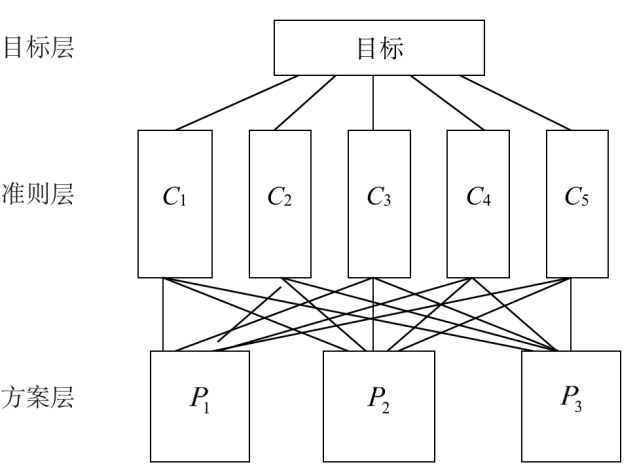
\includegraphics[height=0.25\textheight,width=0.5\linewidth]{figure/q1AHP}%宽度，源文件相对位置
	\caption{层次结构模型图}%图片下方的标题
	\label{fig:q1AHP}%图片引用时所需标签
\end{figure}

\subsubsection{构建层次分析模型}
\noindent \textbf{{\large 构建层次结构}}

首先，构建如下图所示的层次结构图，其中目标层为量化分析企业信贷风险，准则层为守约评分、经营规模、盈利能力、供应侧稳定性、需求侧稳定性、信誉评级六大因素，方案层为123家公司的信贷能力。

\begin{figure}[H]
	\centering
	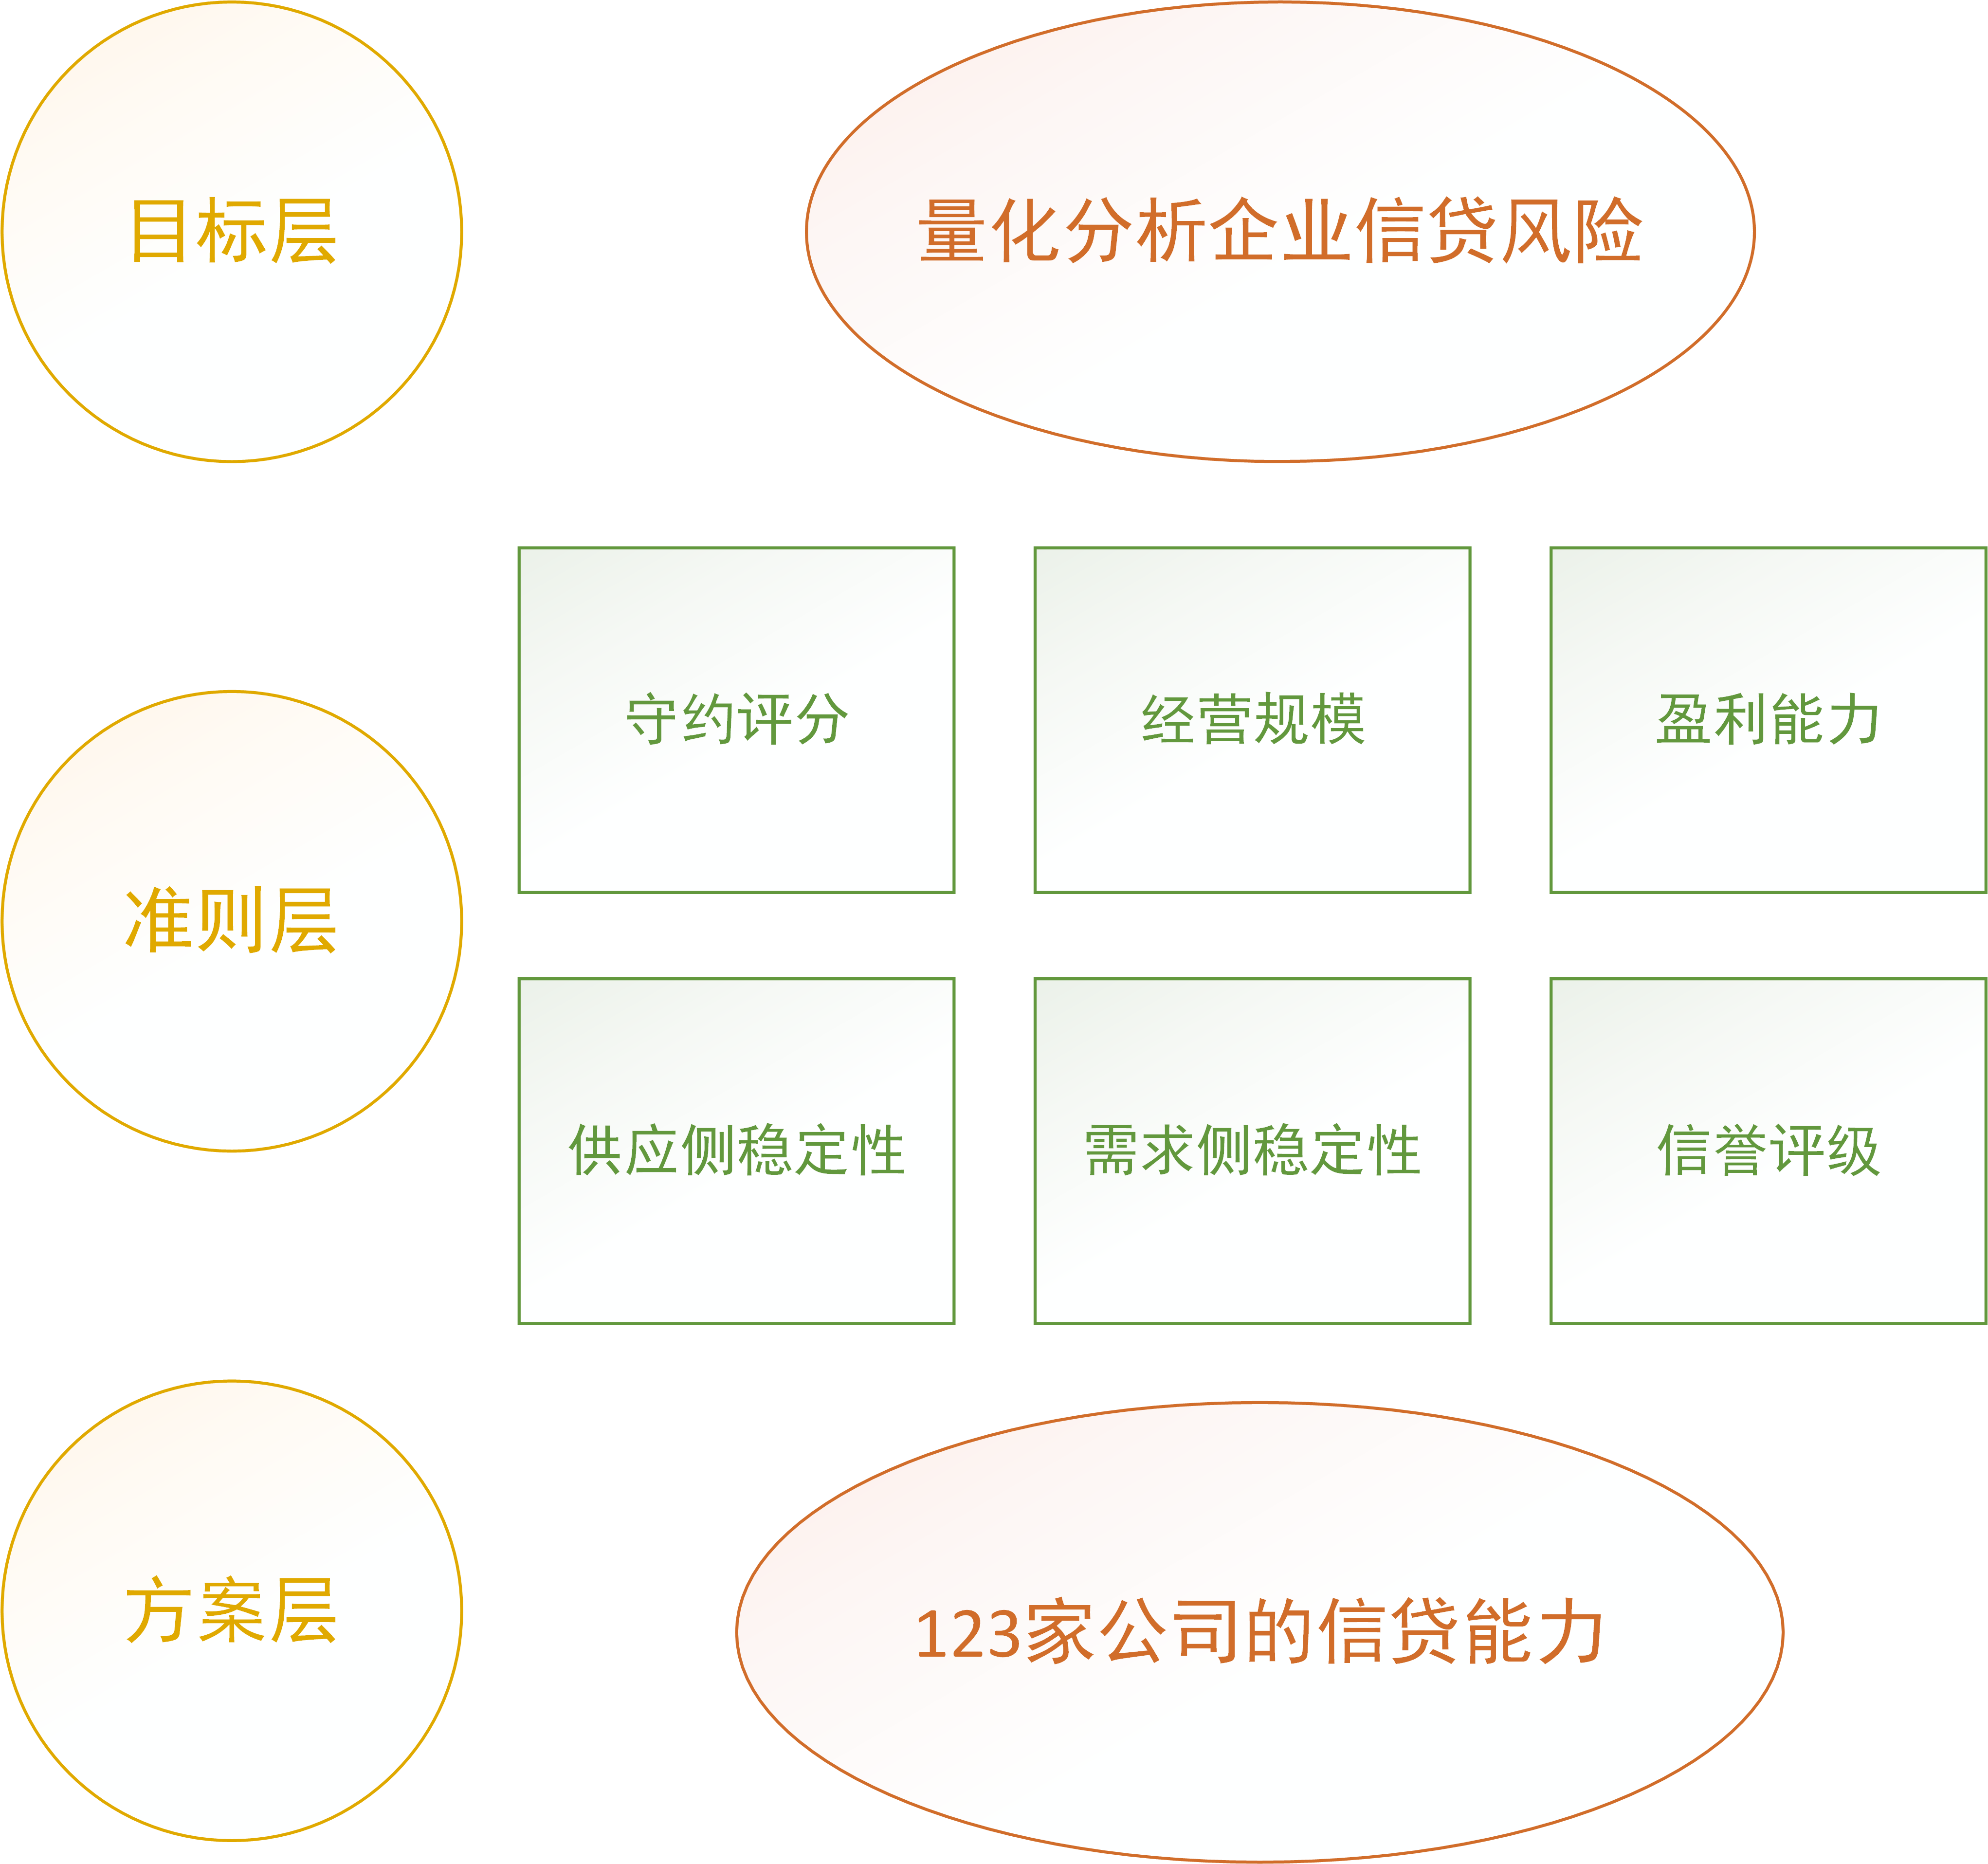
\includegraphics[height=0.25\textheight,width=0.5\linewidth]{figure/q1AHAModel}%宽度，源文件相对位置
	\caption{层次结构图}%图片下方的标题
	\label{fig:q1AHAModel}%图片引用时所需标签
\end{figure}

\noindent \textbf{{\large 构造成对比较矩阵}}

接着，我们通过比较六个因素两两之间相对重要程度，构造出目标层与准则层之间的成对比较矩阵。

\begin{tcolorbox}[breakable]
	\begin{verbatim}
		%目标层与准则层之间的成对比较矩阵
		A =[
		1  8  3  5  6  1; 
		1/8  1  1/7  1/5  1/4  1/8;
		1/3  7  1  3  2  1/3;
		1/5  5  1/3  1  1/3  1/5;
		1/6  4  1/2  3  1  1/4;
		1  8  3  5  4  1;];
	\end{verbatim}
\end{tcolorbox}

\subsubsection{求解层次分析模型}

我们在MATLAB中调用预先编写好的函数\verb|AHP()|，该函数的代码可以在附录中找到。

\begin{tcolorbox}[breakable]
	\begin{verbatim}
		[W, Lmax, CI, CR] = AHP(A)
	\end{verbatim}
\end{tcolorbox}

随后，我们得到如下所示对应的权重向量$ W $、最大特征值$ L_{max} $、一致性指标$ CI $以及一致性比率$ CR $，并通过$ CI $与$ CR $，对所得出的权重向量，进行一致性检验，判断出该权重向量可作为最终的决策依据。

\[\left\{ \begin{array}{l}
		W = {[0.3482;0.0263;0.1475;0.0645;0.0952;0.3182]^{\rm{T}}} \\
		{L_{max}} = 6.3584                                         \\
		CI = 0.0717                                                \\
		CR = 0.0578
	\end{array} \right.\]

应用该权重向量，我们可以计算得出每个企业的信贷能力，如下图所示：

\begin{figure}[H]
	\centering
	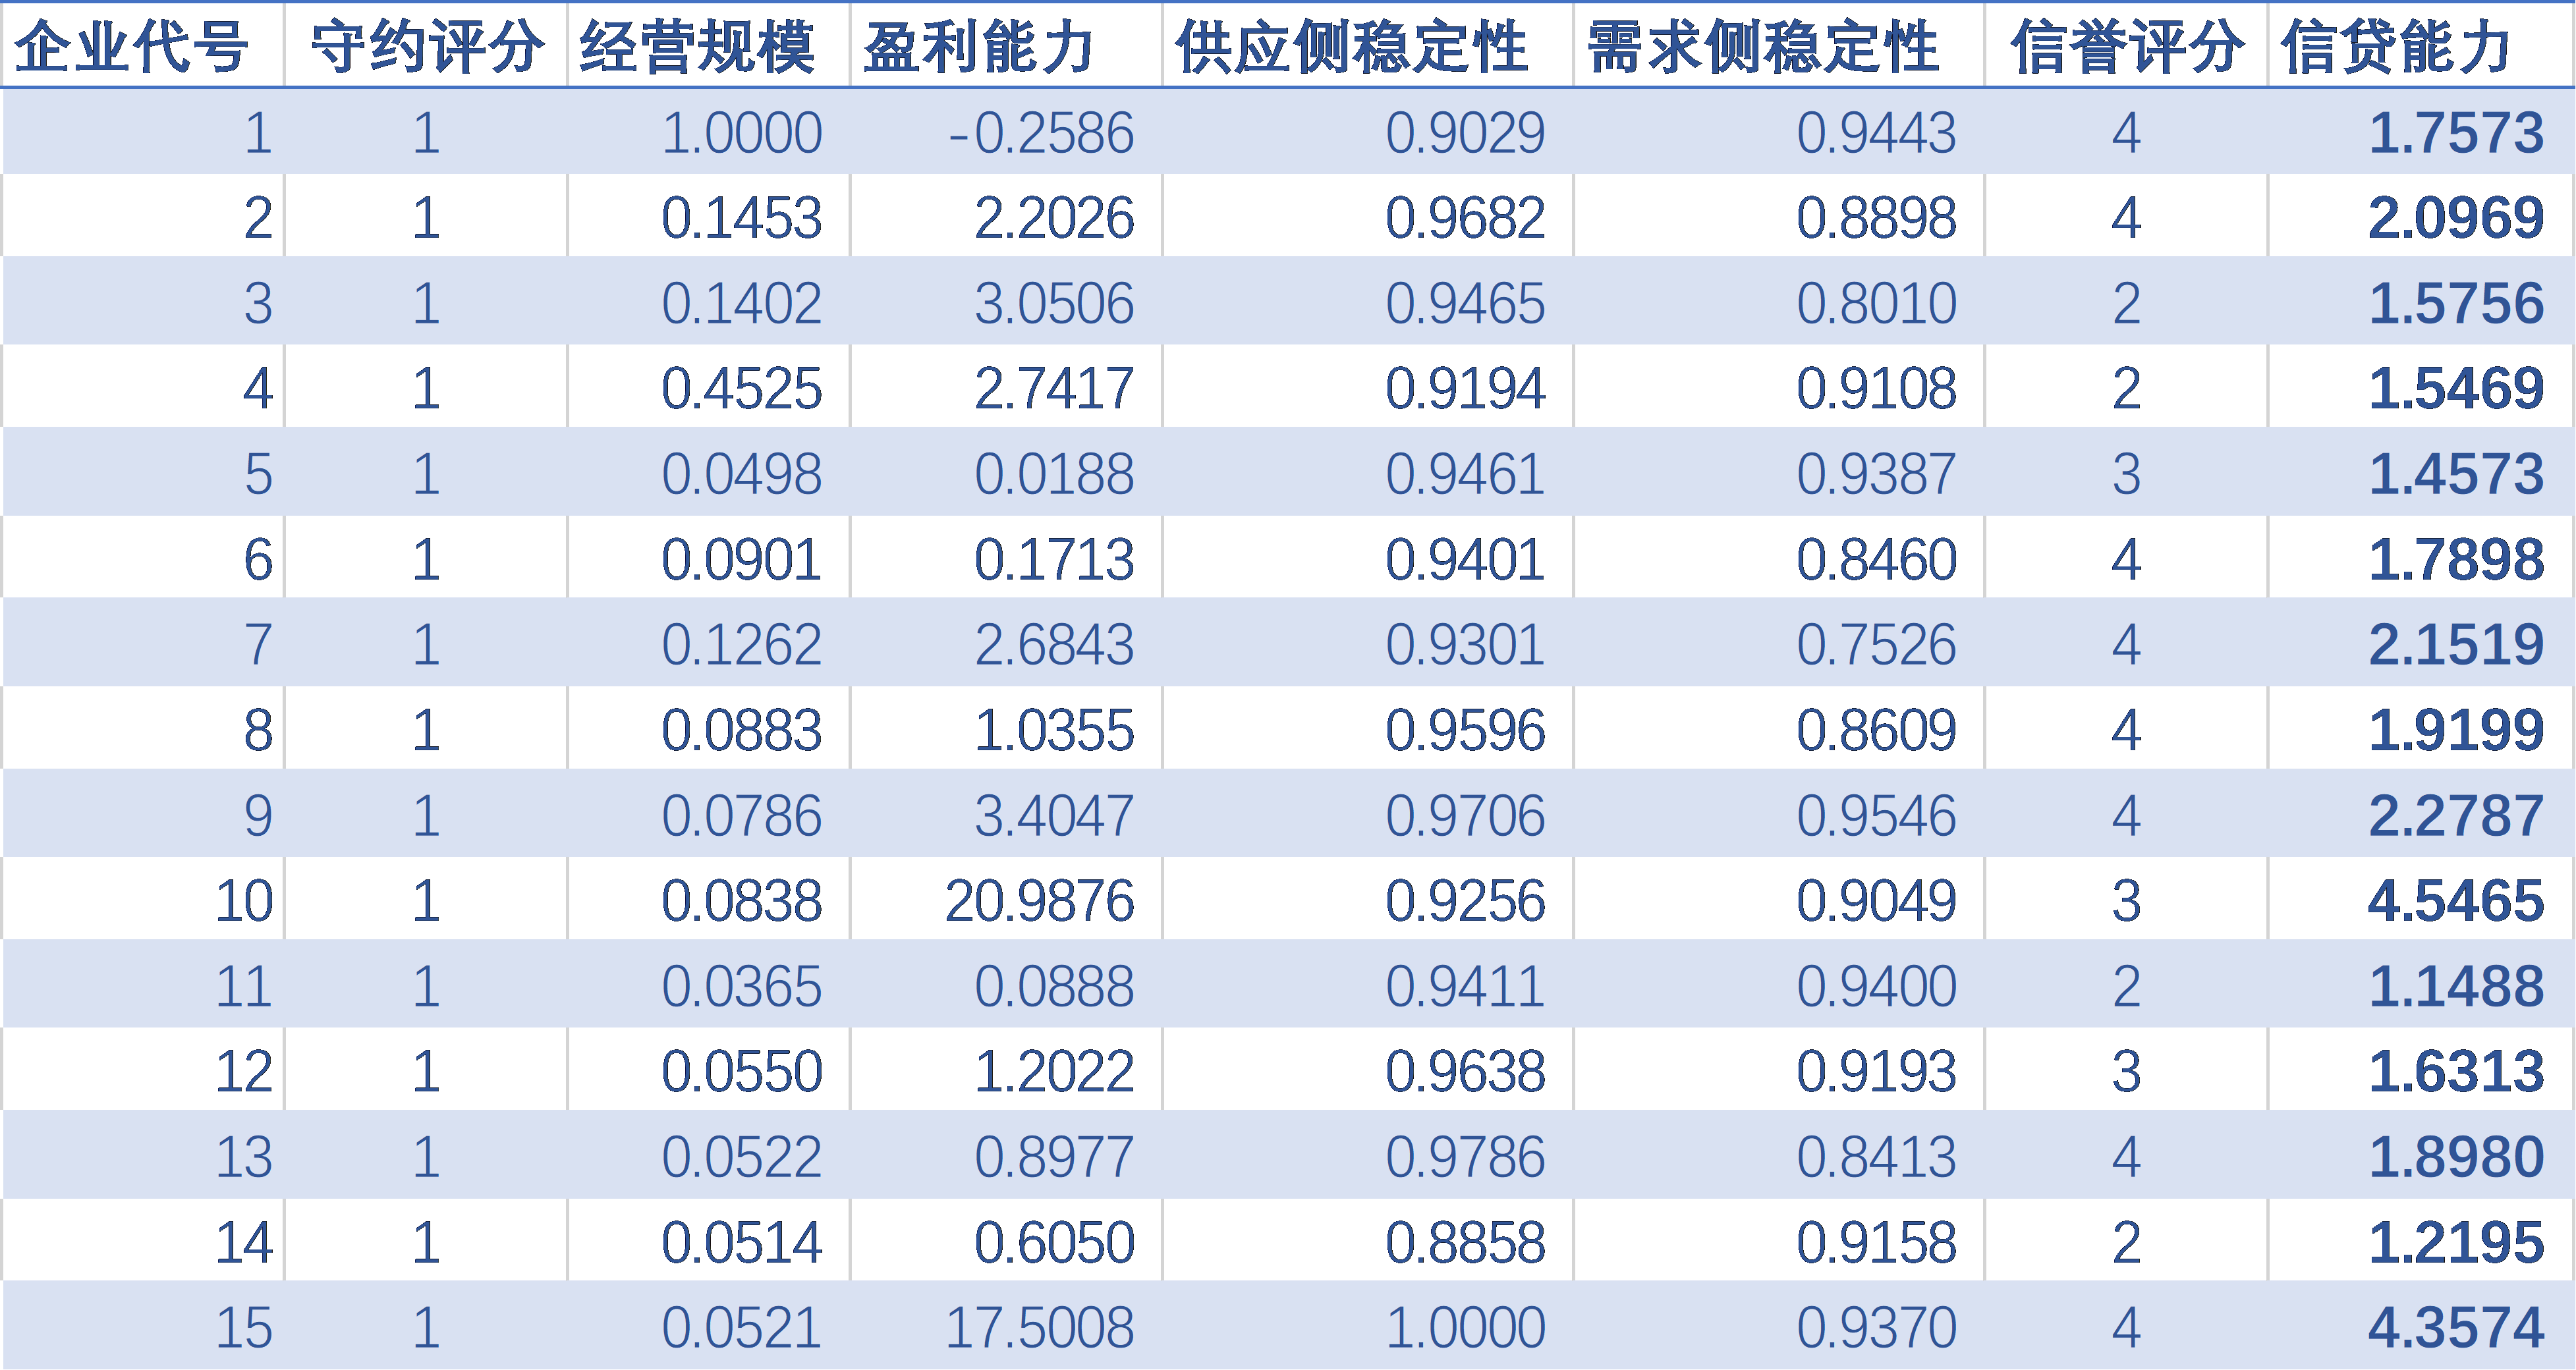
\includegraphics[width=0.5\linewidth]{figure/q1Ability}%宽度，源文件相对位置
	\caption{前15家企业的信贷能力}%图片下方的标题
	\label{fig:q1Ability}%图片引用时所需标签
\end{figure}


\subsubsection{层次分析模型的评价}

通过运用层次分析法，在构造出成对比较矩阵后，调用MATLAB中调用预先编写好的函数，分别计算出对应的权重向量$ W $、最大特征值$ L_{max} $、一致性指标$ CI $，一致性比率$ CR $。

权重向量$ W $，其权系数大小代表相应目标在多目标最优化问题中的重要程度，其值越大表示相应目标在问题中越重要。

最大特征值$ L_{max} $，以此来计算对应的一致性指标$ CI $、一致性比率$ CR $。

一致性指标$ CI $ ，当$ CI = 0 $，有完全的一致性；$ CI $接近于0，有满意的一致性；$ CI $越大，不一致越严重。

一致性比率$ CR $，若$ CR < 0.1 $，认为A的不一致程度在容许范围之内，否则应重新构造成对比较矩阵。

根据上述我们计算所得的结果显示，$ CR < 0.1 $，构造出的成对比较矩阵的不一致程度在容许范围之内，因此认为整个层次的比较判断通过一致性检验，可用上述所得特征向量作为权向量，可按组合权向量表示的结果进行决策。


\subsection{规划求解信贷策略}
\subsubsection{规划求解理论}

在信贷策略模型的建立方面，我们采用了规划求解理论\cite{ref1}以此建立数学模型。在现有的约束条件下，如何充分利用资源，使任务或目标完成得最好。或是在给定目标下，如何以最少的资源消耗，实现这个目标，这便是规划求解理论的主要内容。因此，我们需要根据以下三个步骤建立我们需要的模型：

\begin{enumerate}[1.]
	\item 根据影响所要达到目的的因素找到决策变量；
	\item 由决策变量和所在达到目的之间的函数关系确定目标函数；
	\item 由决策变量所受的限制条件确定决策变量所要满足的约束条件。
\end{enumerate}

\subsubsection{规划模型的构建}

下面是我们根据规划求解理论建立的信贷策略模型。在银行年度信贷总额固定并且每家企业贷款总额之和小于等于银行年度信贷总额的约束条件之下，我们需要使得银行收入的数学期望值达到最高，即可给出该银行在年度信贷总额固定时对这些企业的信贷策略。

在年利率不低于4\%并且不超过15\%，银行给予每家企业贷款额度不低于10万元并且不超过100万元的前提下，我们借助前述所分析出来的数据、信誉评级评分和信贷能力，结合企业的排位百分比，区分银行是否给企业贷款，并将可以贷款的企业的贷款额度和贷款年利率进行分档处理，共分为如下图所示的31种档位。在此分档面板中，我们通过排位百分比，将处于不同档位的企业的贷款额度、贷款年利率作出相应调整，使得实力越强，信誉越高的企业，即所处档位越前的企业，能够获得越大的贷款额度，但不超过100万元，越低的贷款年利率，但不低于4\%，以此达到向实力强、供求关系稳定的企业提供贷款，并对信誉高、信贷风险小的企业给予利率优惠的目的，从而使银行所获收入的数学期望值越高。

\begin{figure}[H]
	\centering
	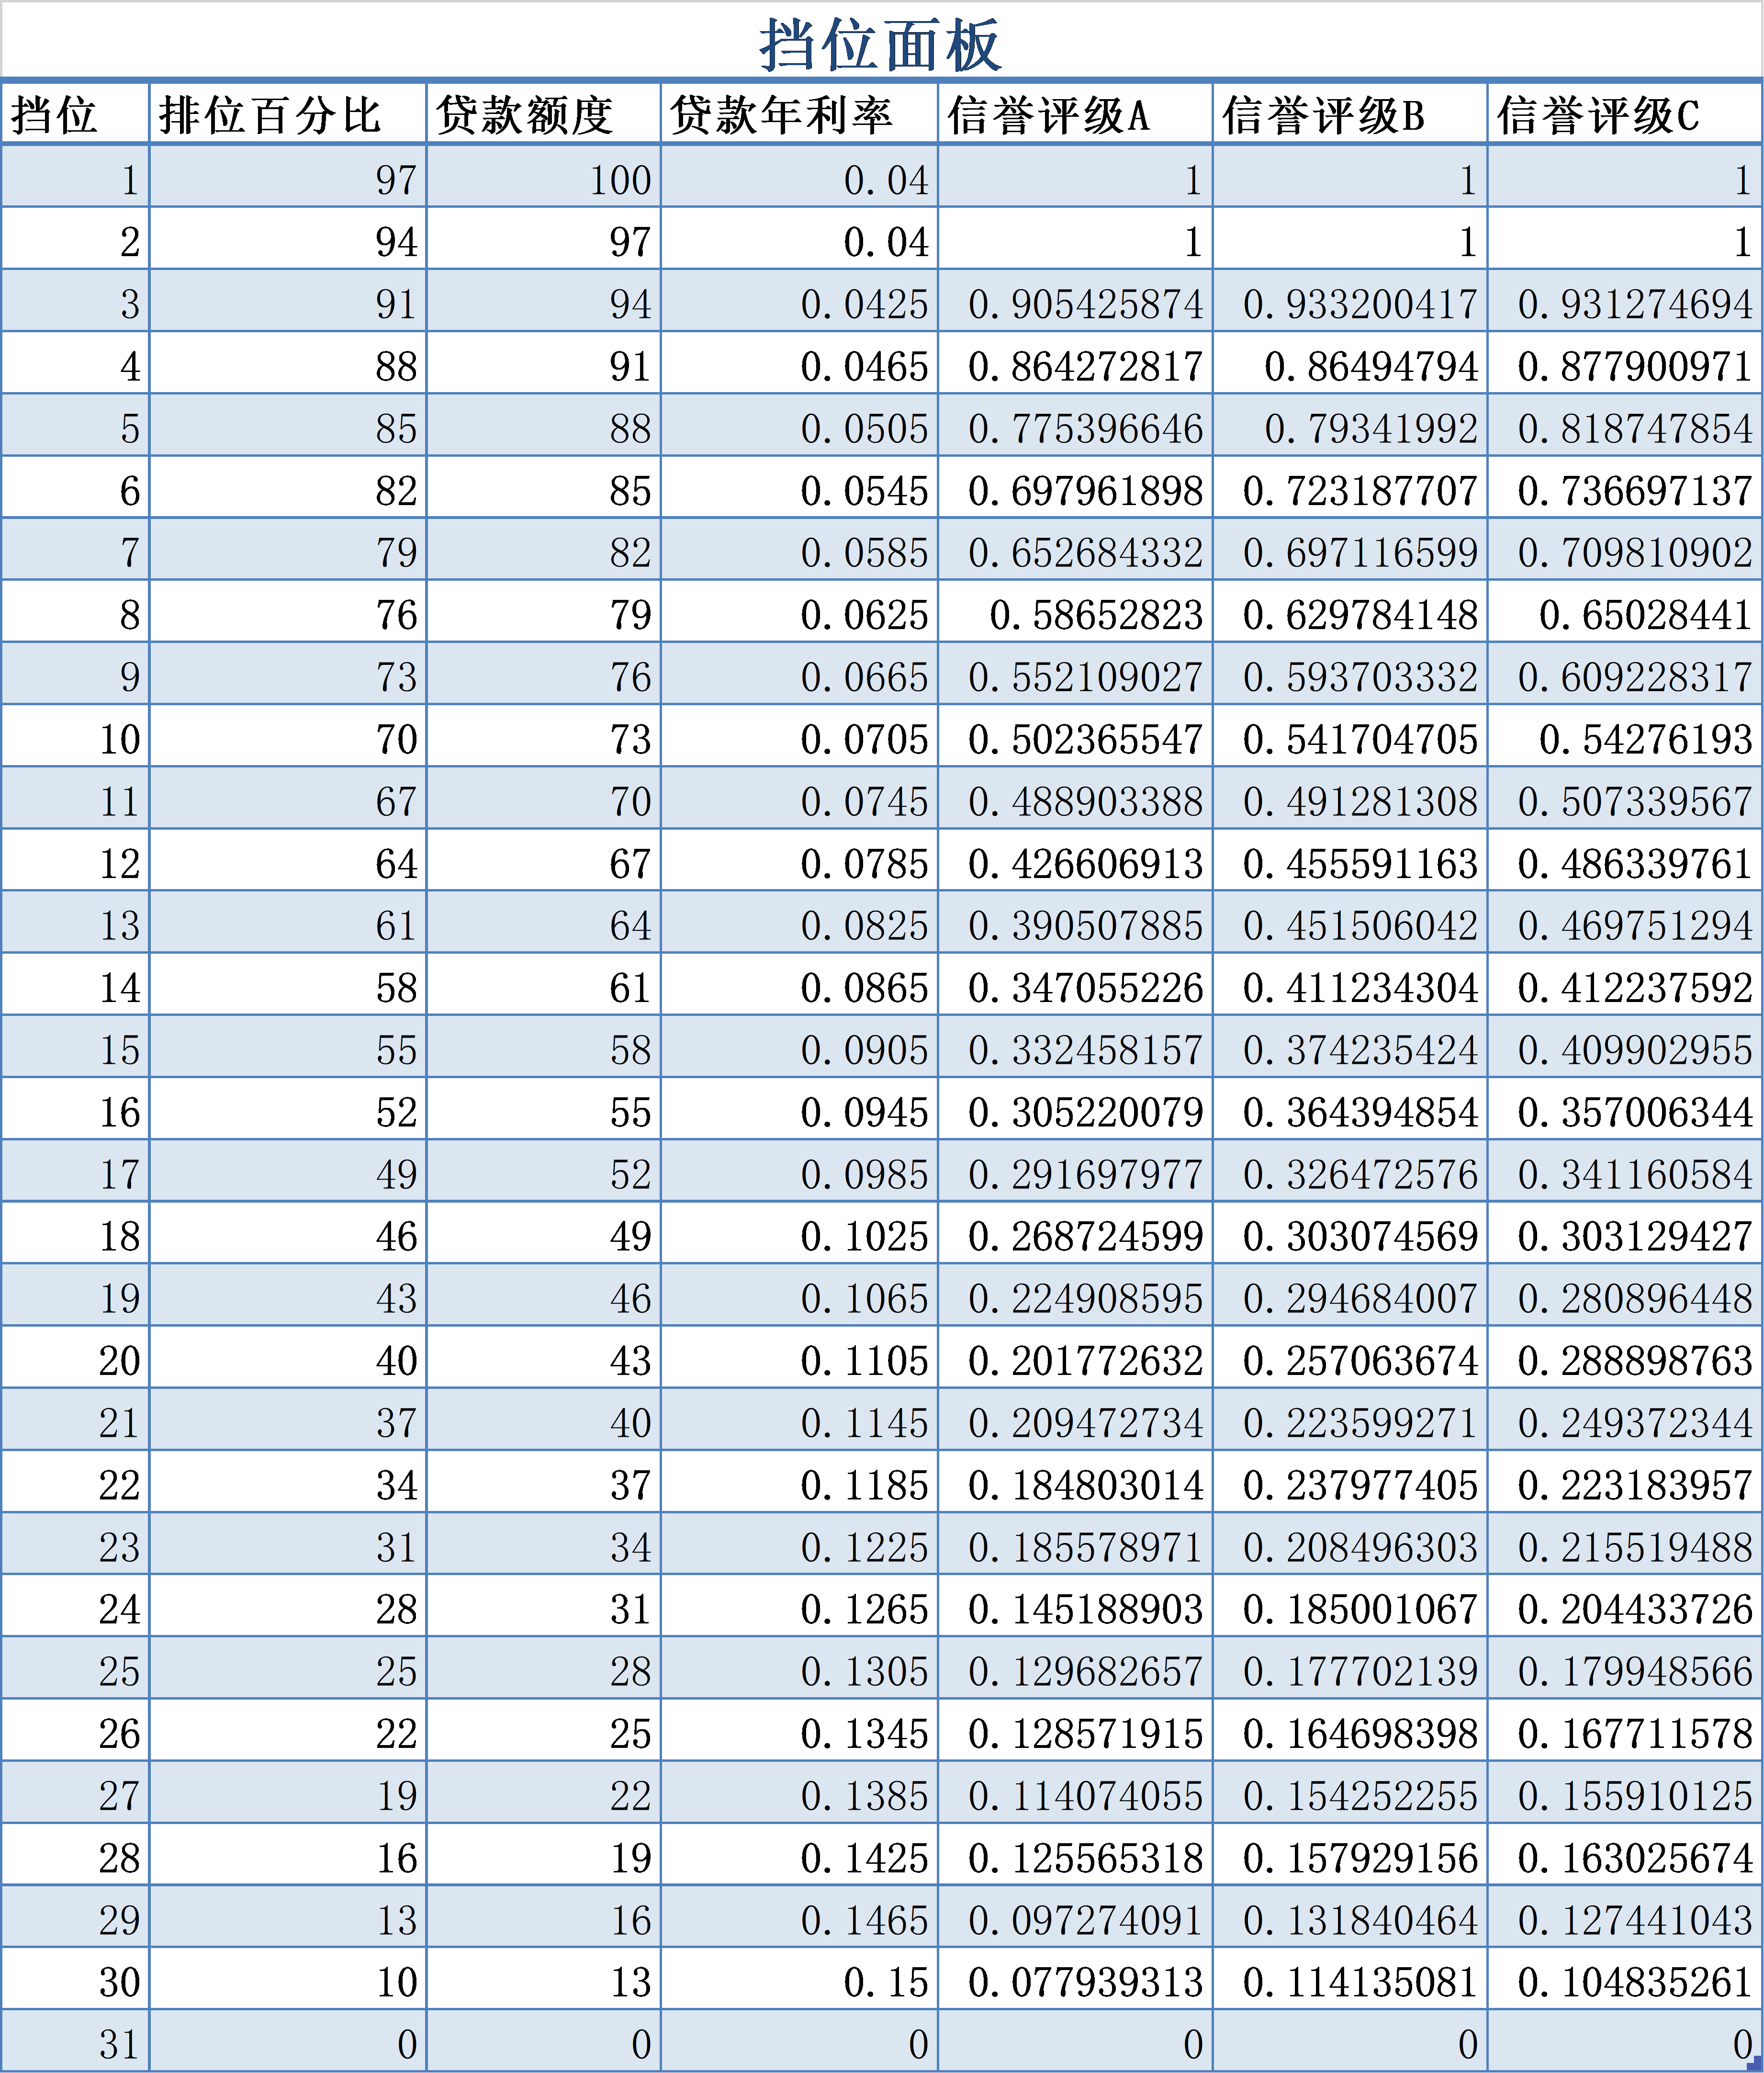
\includegraphics[width=0.5\linewidth]{figure/q1GearPanel}%宽度，源文件相对位置
	\caption{档位面板}%图片下方的标题
	\label{fig:q1GearPanel}%图片引用时所需标签
\end{figure}


\subsubsection{规划模型的求解}

当将企业的贷款额度及年利率加以分档之后，我们借助在MATLAB中预先编写好的代码，导入计算出的企业相关数据，进行相应处理后，调用函数\verb|linprog()|，具体代码可在附录中查看，最后得出在银行年度信贷总额固定时各家企业实际贷款额度。

下面展示随银行信贷总额变化时，部分企业贷款额度的变化数据：

\begin{figure}[H]
	\centering
	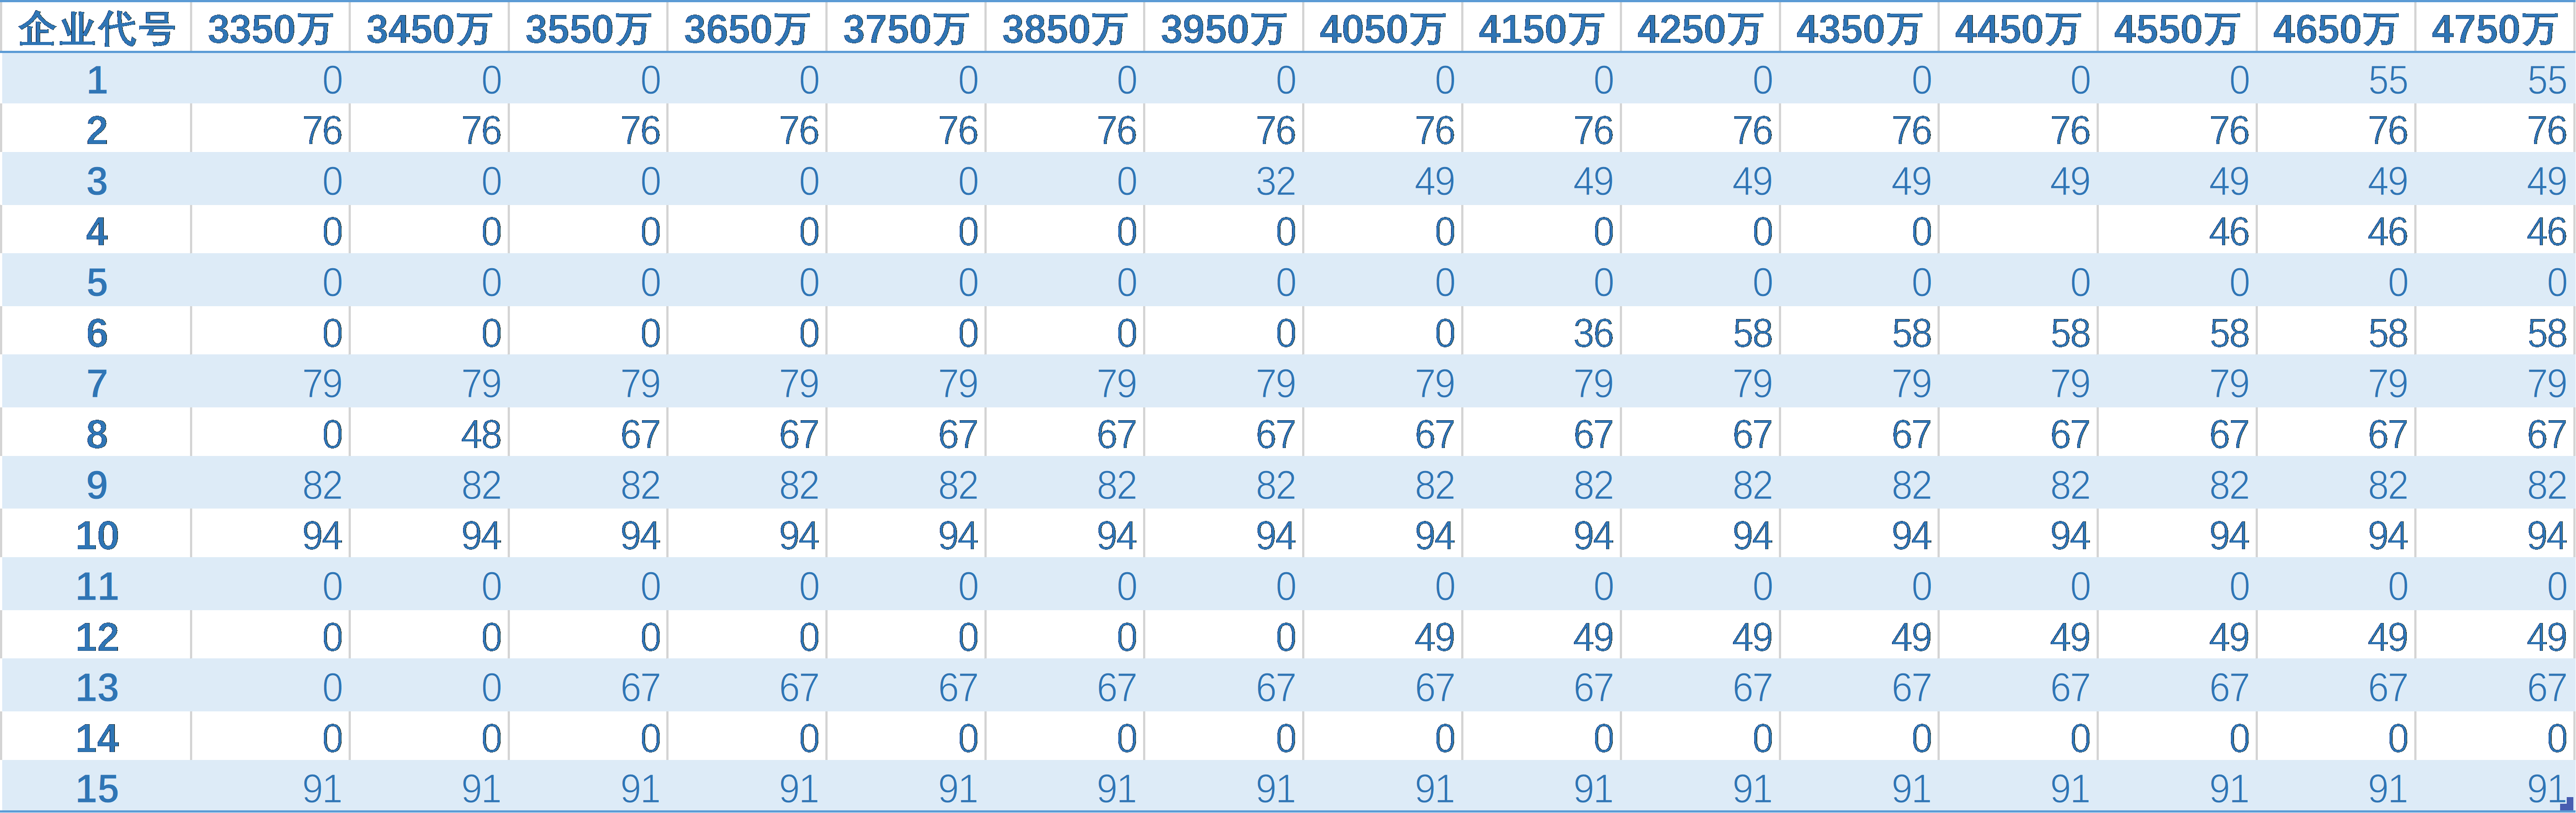
\includegraphics[width=0.75\linewidth]{figure/q1Table}%宽度，源文件相对位置
	\caption{规划求解部分结果}%图片下方的标题
	\label{fig:q1Table}%图片引用时所需标签
\end{figure}

%分文件结束
\ifx\allfiles\undefined
\end{document}
\fi%问题一的建模与分析
\ifx\allfiles\undefined
%生成目录超链接，使用UTF8字符集
\documentclass[12pt,UTF8]{ctexart}


\usepackage{mathtools}%花括号括起的公式
\usepackage{enumerate}%列表
\usepackage{graphicx}%表格
\usepackage[table]{xcolor}%彩色表格
\usepackage{booktabs}%调整表格行高


\renewcommand\tabcolsep{50pt}
\renewcommand\arraystretch{2}

%文本框
\usepackage{tcolorbox}
\tcbuselibrary{skins,vignette,raster,listings,listingsutf8,theorems, breakable,magazine,fitting}

%页面设置
\usepackage{geometry}%设置页面
\usepackage{setspace}%设置局部行距

\usepackage{ctex}
\usepackage{CJK}

%图像处理
\usepackage{graphicx}
\usepackage{float}%允许浮动
\usepackage{caption}%设置标题
\usepackage{graphicx, subfig}

%附录
\usepackage[toc,page]{appendix}

%导言区
\title{中小微企业的信贷决策}

%不要页眉
\pagestyle{plain}
\bibliographystyle{plain}

\geometry{a4paper}%将纸张设置为A4大小

%修改文档结构层次的名称
\usepackage{titlesec}%chapter1修改为一
\titleformat{\part}{\centering\Huge\bfseries}{\thepart}{1em}{}
\renewcommand\thepart{\chinese{part}}

%subsubsubsection的使用
%\usepackage{titlesec}
%\titleclass{\subsubsubsection}{straight}[\subsection]
%
%\newcounter{subsubsubsection}[subsubsection]
%\renewcommand\thesubsubsubsection{\thesubsubsection.\arabic{subsubsubsection}}
%\renewcommand\theparagraph{\thesubsubsubsection.\arabic{paragraph}}
%
%\titleformat{\subsubsubsection}
%{\normalfont\normalsize\bfseries}{\thesubsubsubsection}{1em}{}
%\titlespacing*{\subsubsubsection}
%{0pt}{3.25ex plus 1ex minus .2ex}{1.5ex plus .2ex}
%
%\makeatletter
%\renewcommand\paragraph{\@startsection{paragraph}{5}{\z@}%
%	{3.25ex \@plus1ex \@minus.2ex}%
%	{-1em}%
%	{\normalfont\normalsize\bfseries}}
%\renewcommand\subparagraph{\@startsection{subparagraph}{6}{\parindent}%
%	{3.25ex \@plus1ex \@minus .2ex}%
%	{-1em}%
%	{\normalfont\normalsize\bfseries}}
%\def\toclevel@subsubsubsection{4}
%\def\toclevel@paragraph{5}
%\def\toclevel@paragraph{6}
%\def\l@subsubsubsection{\@dottedtocline{4}{7em}{4em}}
%\def\l@paragraph{\@dottedtocline{5}{10em}{5em}}
%\def\l@subparagraph{\@dottedtocline{6}{14em}{6em}}
%\makeatother
%
%\setcounter{secnumdepth}{4}

\begin{document}
\else
\fi
%分文件开始


\section{问题二模型的建立和求解}
\subsection{构建进行信誉评级的决策树模型}
\subsubsection{决策树理论简介}

下面我们简要介绍一下决策树理论\cite{ref2}。所谓决策树，顾名思义，是一种为了解决分类问题依托策略抉择而建立起来的树。通过采用树形结构，使用层层推理来实现最终的分类。通常决策树包含下面三种主要元素，一是根节点，其包含样本的全集；二是内部节点，其对应特征属性的测试；三是叶节点，其代表决策的结果。

\begin{figure}[htbp]
	\centering
	\begin{minipage}[t]{0.49\linewidth}
		\centering
		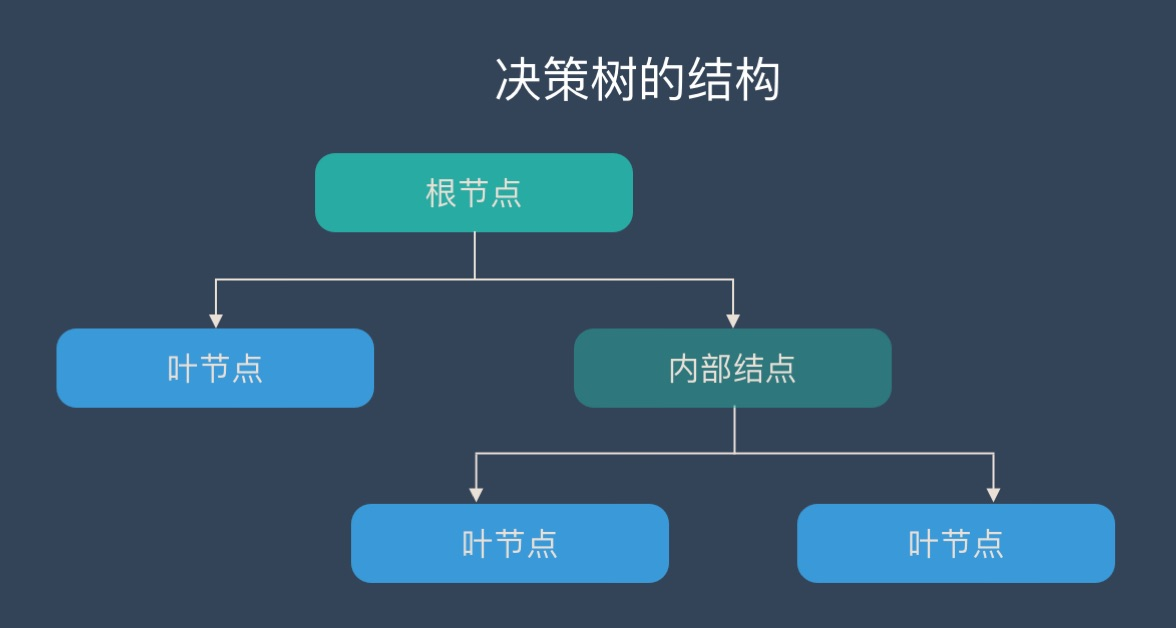
\includegraphics[height=0.15\textheight,width=0.75\linewidth]{figure/q2DecisionMakingTree1}%宽度，源文件相对位置
		\caption{决策树的结构}%图片下方的标题
	\end{minipage}
	\begin{minipage}[t]{0.49\textwidth}
		\centering
		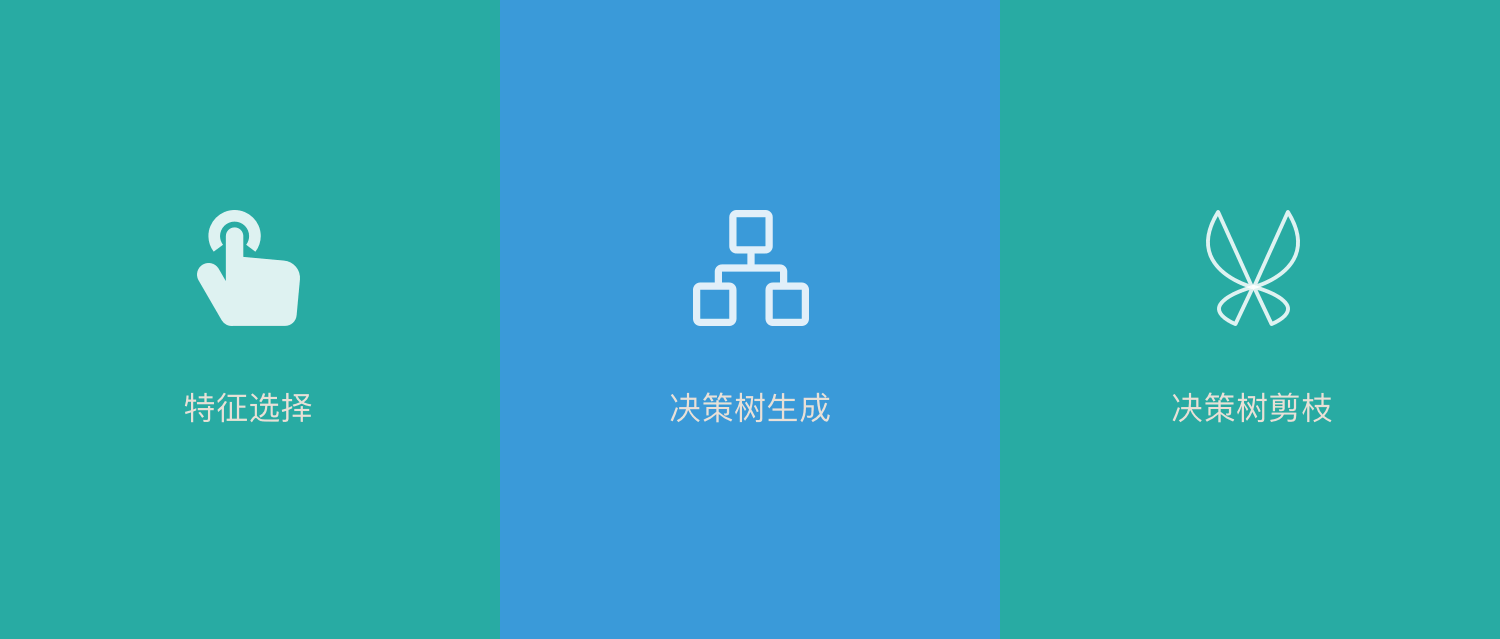
\includegraphics[height=0.15\textheight,width=0.75\linewidth]{figure/q2DecisionMakingTree2}%宽度，源文件相对位置
		\caption{决策树学习三步骤}%图片下方的标题
	\end{minipage}
\end{figure}

在运用决策树理论\cite{ref2}的过程中，首先需根据信息增益的原则，进行特征选择，从而筛选出跟分类结果相关性较高的特征。接着从根节点触发，对节点计算所有特征的信息增益，选择信息增益最大的特征作为节点特征，并根据该特征的不同取值建立子节点。之后对每个子节点使用相同的方式生成新的子节点，直到信息增益很小或者没有特征可以选择为止，进而生成决策树。最后对已生成好的决策树进行剪枝，通过主动去掉部分分支来降低过拟合的风险，得到最终分类结果。

\subsubsection{据已有信誉评级训练决策树模型}

在建立决策树模型过程中，我们通过MPai数据科学平台来训练决策树。所谓MPai数据科学平台是一款基础性数据分析软件，以低门槛、一站式、规范化、高效率为主要特征，使我们能够快速掌握数据分析。在MPai平台，我们首先创建一个工程来存放数据与分析结果，接着我们将数据导入相应文件夹，之后我们配置决策树模型，根据已有信誉评级设置如下表所示的相应工程参数，最后便可在分析结果页查看最终训练结果，快速得出最拟合数据的模型特征概要。


根据如上表格设置相应参数后进行求解，所得到的结果如下：

\begin{figure}[H]
	\centering
	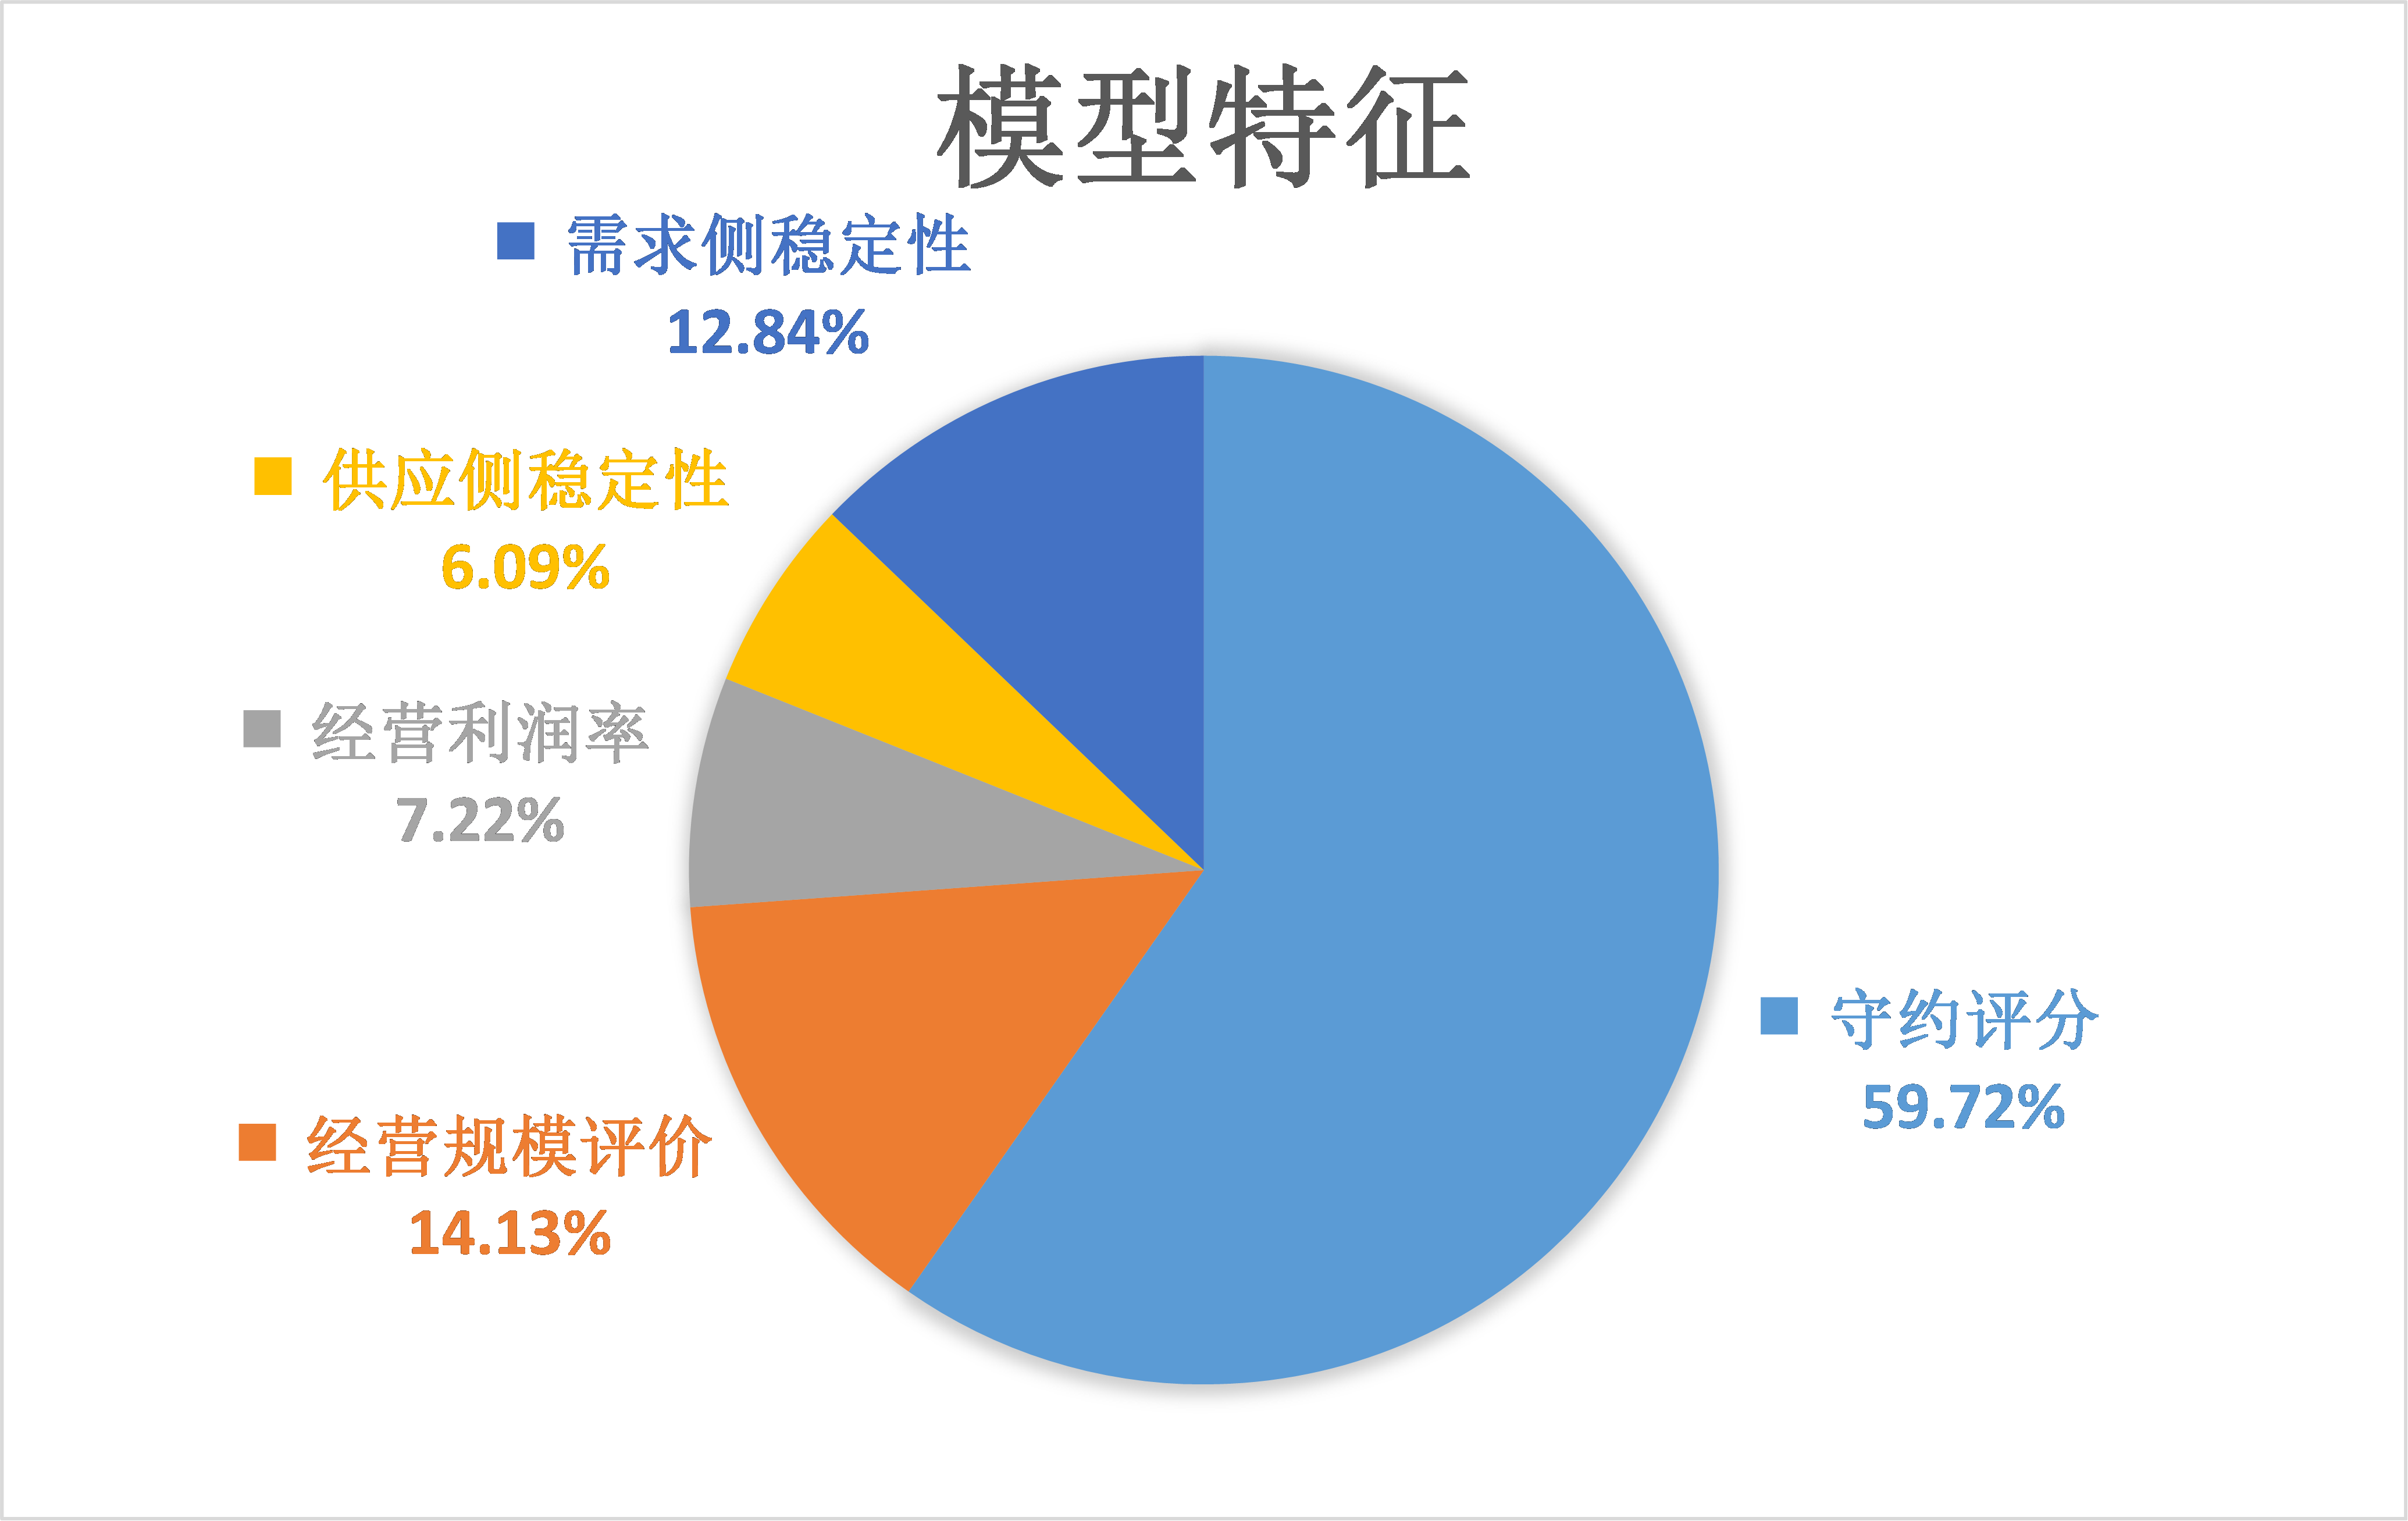
\includegraphics[width=0.75\linewidth]{figure/q2ModelAnalysis}%宽度，源文件相对位置
	\caption{模型特征}%图片下方的标题
	\label{fig:q2ModelAnalysis}%图片引用时所需标签
\end{figure}

\subsubsection{决策树模型的评价}

在模型建立方面，我们通过在MPai数据科学平台上训练决策树，得到如下评估结果，评价指标包括$ MSE $，$ RMSE $，$ MAE $，$ R^{2} $，$ MAPE $\cite{ref2}。

$ MSE $即均方误差，范围[0,+∞) ，当预测值与真实值完全吻合时等于0，即完美模型；误差越大，该值越大。

$ RMSE $即均方根误差，范围[0,+∞)，当预测值与真实值完全吻合时等于0，即完美模型；误差越大，该值越大。

$ MAE $即平均绝对误差，范围[0,+∞)，当预测值与真实值完全吻合时等于0，即完美模型；误差越大，该值越大。

$ R^{2} $即相关系数，范围[0,1]，是一个评价拟合好坏的指标。一般来说，$ R^{2} $越大，表示模型拟合效果越好。

$ MAPE $即平均绝对百分比误差，范围[0,+∞)，等于$0\%$表示完美模型，大于  $100\%$则表示劣质模型。

由我们得到的评估结果如下表所示，说明我们的模型建立的预测值与真实值的误差很小，是几乎吻合的。

\begin{center}
	\begin{table}[H]  %table 里面也可以嵌套tabular,只有tabular是不能加标题的
		\centering
		\caption{测试数据评估结果}  %表格标题
		\resizebox{250pt}{75pt}{
			\begin{tabular}{cr}
				\hline
				评价指标  & 评价结果 \\
				\hline
				$ MSE $   & 60.6317  \\
				$ RMSE $  & 7.7866   \\
				$ MAE $   & 34.6613  \\
				$ R^{2} $ & 0.3807   \\
				$ MAPE $  & 55.9964  \\
				\hline
			\end{tabular}}
	\end{table}
\end{center}


\subsection{量化分析信贷风险}
\subsubsection{用决策树模型进行信誉评级}

利用MPai数据科学平台配置好决策树模型后，将前述处理得到的302家企业的各项指标数据导入创建好的工程中，并在结果页查看最终预测结果。下面展示了利用决策树模型处理得到的前10个数据的预测结果：

\begin{center}
	\begin{table}[H]  %table 里面也可以嵌套tabular,只有tabular是不能加标题的
		\centering
		\caption{决策树模型各指标前10个数据展示}  %表格标题
		\resizebox{300pt}{75pt}{
			\begin{tabular}{ccrrrr}
				\hline
				预测结果Y & 守约评分 & 经营规模评分 & 经营利润率 & 供应侧稳定性 & 需求供应侧稳定性 \\
				\hline
				4.00      & 1        & 0.7881       & -0.0652    & 0.8411       & 0.8183           \\
				4.00      & 1        & 1.0000       & -0.0063    & 0.8406       & 0.8389           \\
				2.00      & 1        & 0.5532       & 3.5657     & 0.9550       & 0.8127           \\
				4.00      & 1        & 0.6926       & 29.9004    & 0.9793       & 0.9687           \\
				2.00      & 1        & 0.2575       & 13.4326    & 0.9634       & 0.9251           \\
				4.00      & 1        & 0.3451       & 1.7936     & 0.9285       & 0.8759           \\
				3.00      & 1        & 0.1169       & 0.4182     & 0.9496       & 0.9407           \\
				3.50      & 1        & 0.2221       & 0.6050     & 0.8858       & 0.9158           \\
				3.67      & 1        & 0.2160       & 1.6892     & 0.9750       & 0.9182           \\
				3.67      & 1        & 0.1207       & 1.7742     & 0.9696       & 0.8059           \\
				\hline
			\end{tabular}}
	\end{table}
\end{center}


\subsubsection{用层次分析法量化分析信贷风险}

首先，构建与问题一相类似的层次结构图\cite{ref1}，将决策目标，即目标层，定为量化分析企业信贷风险；决策准则，即准则层，定为守约评分、经营规模、盈利能力、供应侧稳定性、需求侧稳定性、信誉评级六个因素；决策对象，即方案层，定为302家公司的信贷能力。

其次，采用相对尺度法，通过比较六个因素两两之间的相对重要程度，构造出量化分析企业信贷风险，即目标层，与六个因素，即准则层，之间的成对比较矩阵。

然后，我们在MATLAB中调用预先编写好的函数\verb|AHP()|，该函数的代码可以在附录中找到。接着便可得到对应的权重向量$ W $、最大特征值$ L_{max} $、一致性指标$ CI $以及一致性比率$ CR $。利用$ CI $与$ CR $，对所得出的权重向量，进行一致性检验，判断出该权重向量可作为最终的决策依据。

最后运用该权重向量，分别计算出302家企业各自的信贷能力，以此来分析其信贷风险。

\begin{figure}[H]
	\centering
	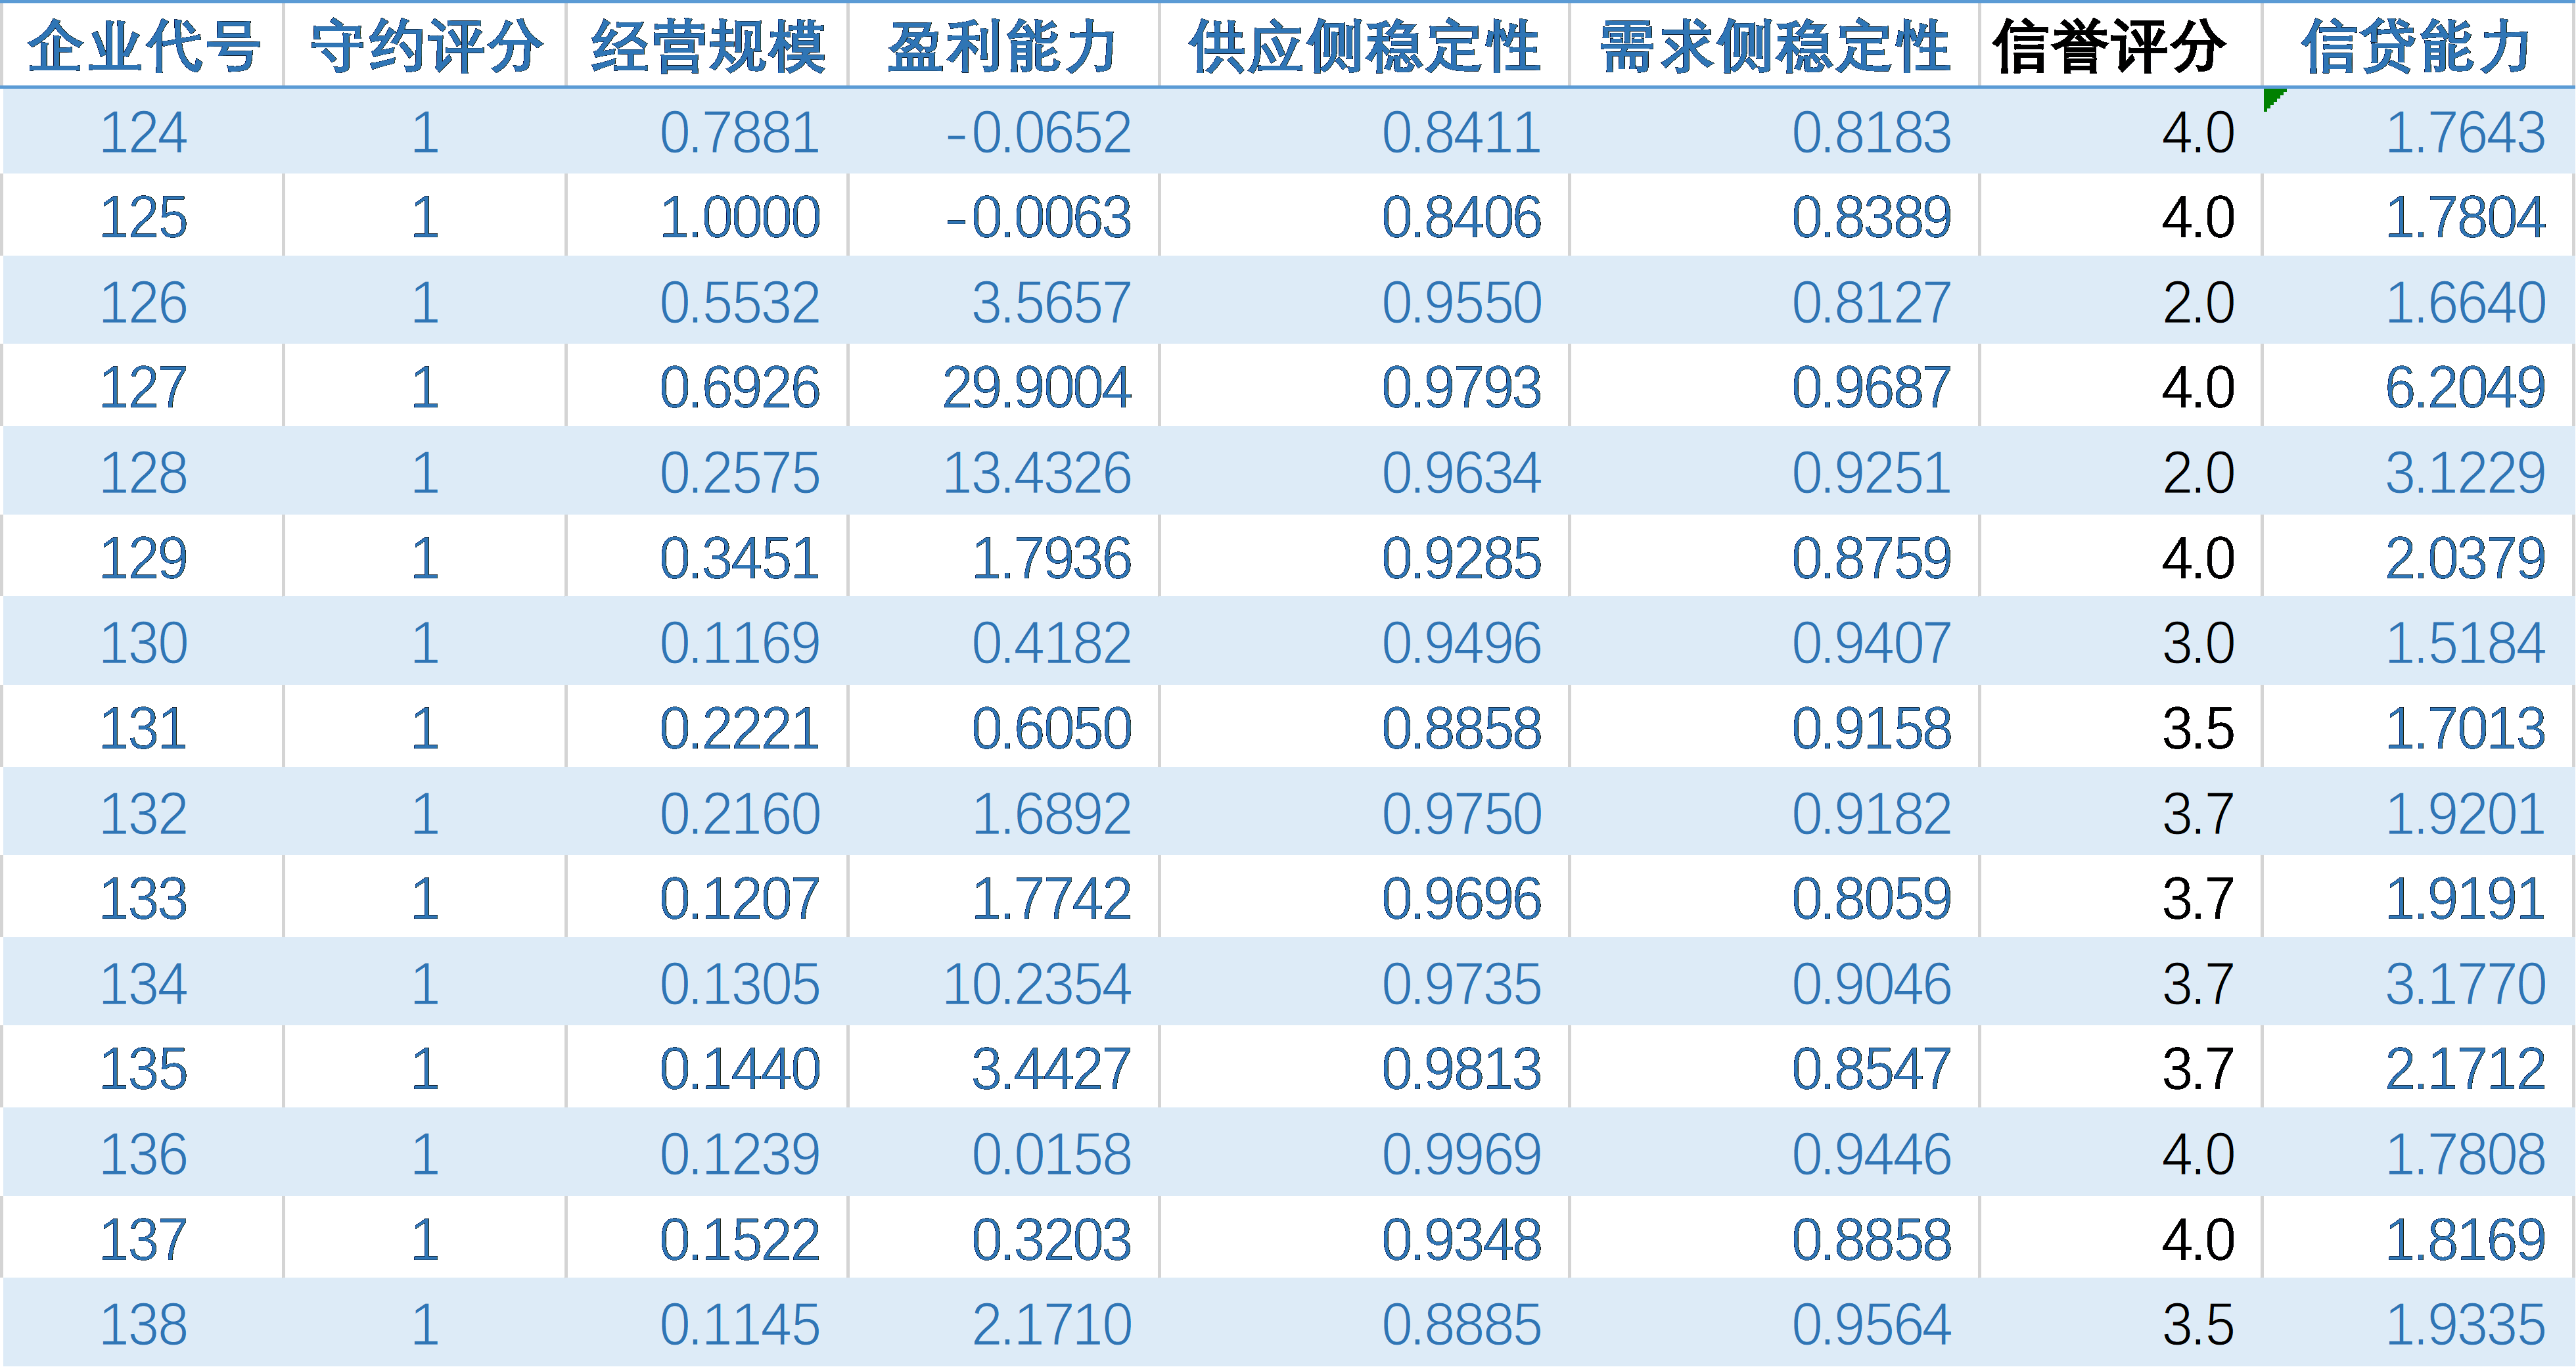
\includegraphics[width=0.75\linewidth]{figure/q2PredictData}%宽度，源文件相对位置
	\caption{部分企业的信贷能力}%图片下方的标题
	\label{fig:q2PredictData}%图片引用时所需标签
\end{figure}

\subsection{规划求解信贷策略}
\subsubsection{规划模型的求解}
在银行年度信贷总额为1亿的约束条件下，我们根据规划求解理论\cite{ref1}建立的信贷策略模型，使银行收入的数学期望值达到最高，即可给出该银行在年度信贷总额为1亿时对这些企业的信贷策略。这里的银行收入的数学期望值就是我们的目标函数。

具体方法同问题一的规划求解方法。首先，在年利率和贷款额度约束条件下，我们结合企业的排位百分比，区分银行是否发放贷款，并将可以贷款的企业的贷款额度和贷款年利率分为与问题一相同的31种档位。接着，我们借助在MATLAB中预先编写好的代码，导入计算出的企业相关数据，并调用函数\verb|linprog()|，具体代码可在附录中查看，得出302家企业实际贷款额度，制定出在银行年度信贷总额为1亿的情况下最为理想的信贷策略。具体结果策略如下图所示。所得银行收入的数学期望值$5.0157 \times {10^4}$。

\begin{figure}[H]
	\centering
	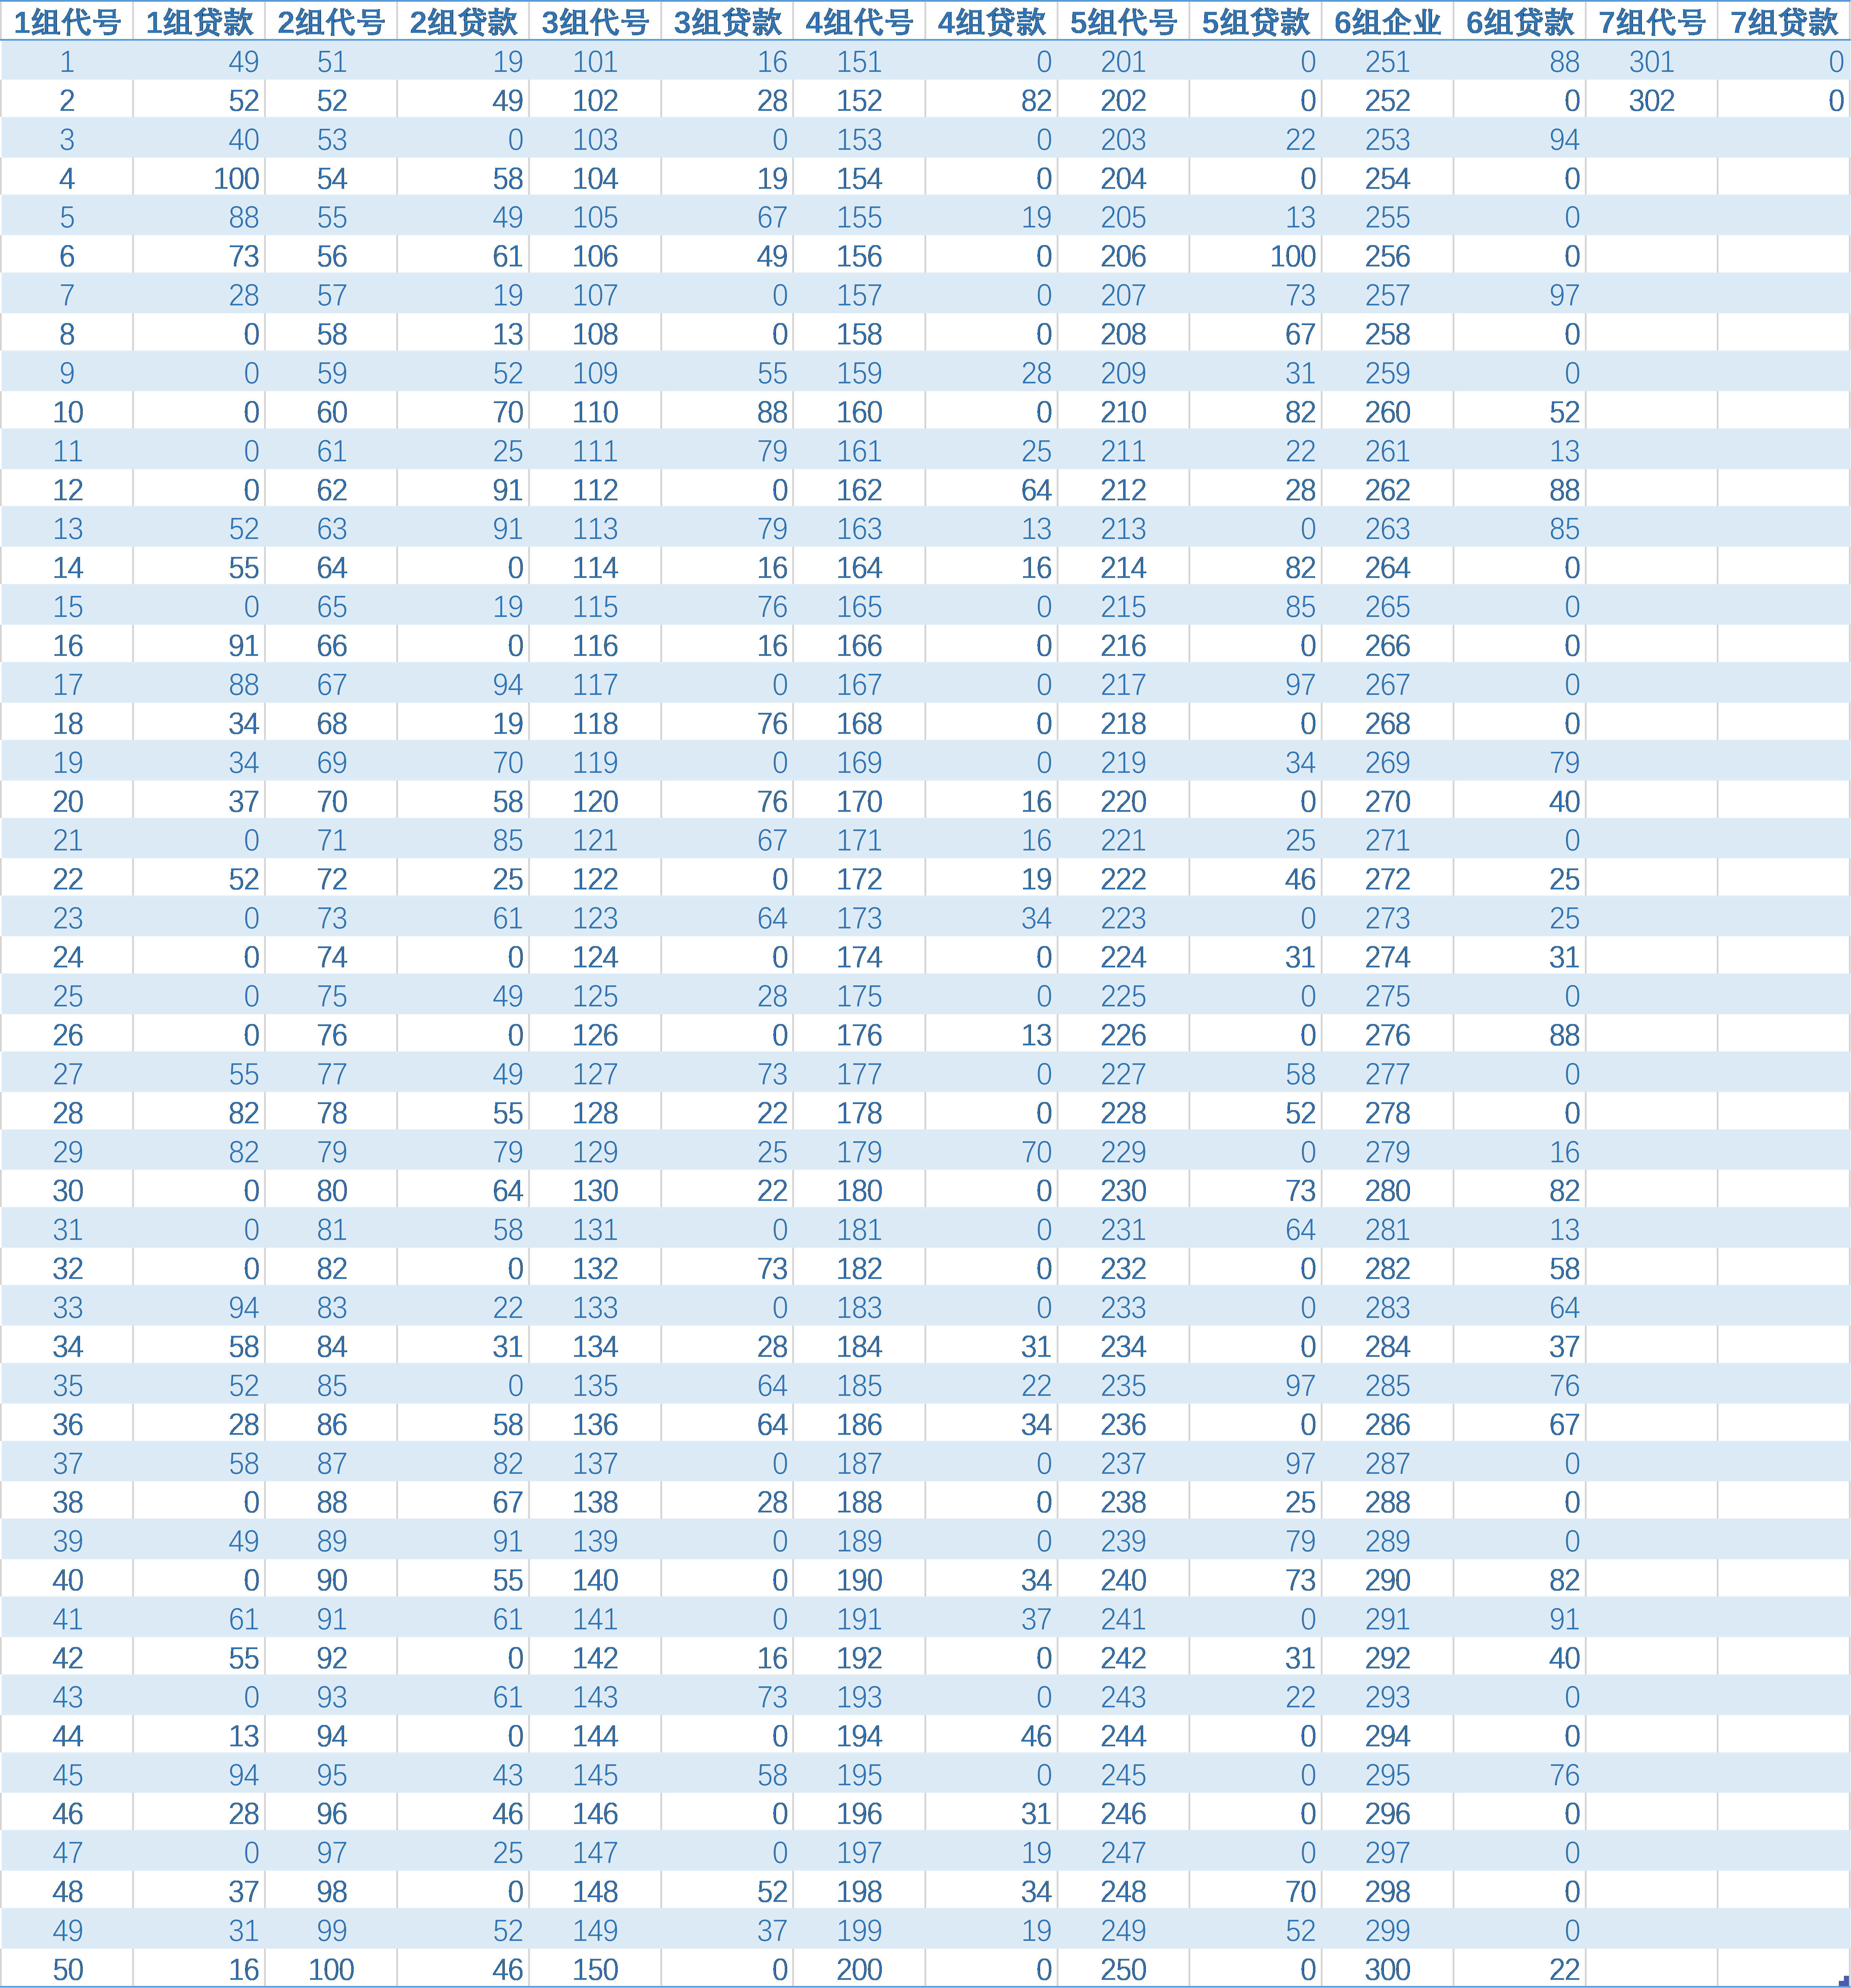
\includegraphics[width=0.75\linewidth]{figure/q2ResultTable}%宽度，源文件相对位置
	\caption{规划求解所得的信贷策略}%图片下方的标题
	\label{fig:q2ResultTable}%图片引用时所需标签
\end{figure}







%分文件结束
\ifx\allfiles\undefined
\end{document}
\fi%问题二的建模与分析
\ifx\allfiles\undefined
%生成目录超链接，使用UTF8字符集
\documentclass[12pt,UTF8]{ctexart}


\usepackage{mathtools}%花括号括起的公式
\usepackage{enumerate}%列表
\usepackage{graphicx}%表格
\usepackage[table]{xcolor}%彩色表格
\usepackage{booktabs}%调整表格行高


\renewcommand\tabcolsep{50pt}
\renewcommand\arraystretch{2}

%文本框
\usepackage{tcolorbox}
\tcbuselibrary{skins,vignette,raster,listings,listingsutf8,theorems, breakable,magazine,fitting}

%页面设置
\usepackage{geometry}%设置页面
\usepackage{setspace}%设置局部行距

\usepackage{ctex}
\usepackage{CJK}

%图像处理
\usepackage{graphicx}
\usepackage{float}%允许浮动
\usepackage{caption}%设置标题
\usepackage{graphicx, subfig}

%附录
\usepackage[toc,page]{appendix}

%导言区
\title{中小微企业的信贷决策}

%不要页眉
\pagestyle{plain}
\bibliographystyle{plain}

\geometry{a4paper}%将纸张设置为A4大小

%修改文档结构层次的名称
\usepackage{titlesec}%chapter1修改为一
\titleformat{\part}{\centering\Huge\bfseries}{\thepart}{1em}{}
\renewcommand\thepart{\chinese{part}}

%subsubsubsection的使用
%\usepackage{titlesec}
%\titleclass{\subsubsubsection}{straight}[\subsection]
%
%\newcounter{subsubsubsection}[subsubsection]
%\renewcommand\thesubsubsubsection{\thesubsubsection.\arabic{subsubsubsection}}
%\renewcommand\theparagraph{\thesubsubsubsection.\arabic{paragraph}}
%
%\titleformat{\subsubsubsection}
%{\normalfont\normalsize\bfseries}{\thesubsubsubsection}{1em}{}
%\titlespacing*{\subsubsubsection}
%{0pt}{3.25ex plus 1ex minus .2ex}{1.5ex plus .2ex}
%
%\makeatletter
%\renewcommand\paragraph{\@startsection{paragraph}{5}{\z@}%
%	{3.25ex \@plus1ex \@minus.2ex}%
%	{-1em}%
%	{\normalfont\normalsize\bfseries}}
%\renewcommand\subparagraph{\@startsection{subparagraph}{6}{\parindent}%
%	{3.25ex \@plus1ex \@minus .2ex}%
%	{-1em}%
%	{\normalfont\normalsize\bfseries}}
%\def\toclevel@subsubsubsection{4}
%\def\toclevel@paragraph{5}
%\def\toclevel@paragraph{6}
%\def\l@subsubsubsection{\@dottedtocline{4}{7em}{4em}}
%\def\l@paragraph{\@dottedtocline{5}{10em}{5em}}
%\def\l@subparagraph{\@dottedtocline{6}{14em}{6em}}
%\makeatother
%
%\setcounter{secnumdepth}{4}

\begin{document}
\else
\fi
%分文件开始


\section{模型的完善与问题三的求解}
\subsection{据行业类别判定疫情对企业经营的影响}
在调查了大量新闻\cite{ref3}的基础上，我们发现：在疫情的冲击下，阻碍各行业发展的主要原因大致有如下三点：一是整体需求萎缩；二是生产要素（如劳动力资源）大量减少或成本上升；三是政策性影响。我们将附件2中的302家企业分为13个行业，并且基于新冠病毒疫情对这些企业的影响程度，将这13个行业分为有利、基本无影响、不利与非常不利4类。

对于个体经营户、工业、建筑业、交通运输业、商品贸易业等行业，需求的萎缩、劳动力资源的减少及经营成本的上升，使得这些企业可能无法正常还贷。对于房地产、服务业、农业、批发零售业、文化艺术业、制造业等行业的企业成本相较于上类企业并没有大幅上升，将会恢复贷款偿还能力。信息传输业行业致力于科研且受到政府支持，所以在疫情影响下相较于上述两类企业来说基本无影响，仍能正常还贷。而医疗业对疫情的防控发挥了巨大的作用，加之政策支持，会提高企业的贷款偿还能力。



\subsection{考虑疫情影响下对信贷风险的量化分析}

我们采用层次分析法\cite{ref1}，对受疫情影响下302家企业的信贷风险进行量化分析。首先，构建出与前述问题类似的层次结构图。然后我们通过比较五个因素两两之间的相对重要程度，构造出目标层与准则层之间的成对比较矩阵。接着我们在MATLAB中调用预先编写好的函数\verb|AHP()|，该函数的代码可以在附录中找到。

\begin{tcolorbox}[breakable]
	\begin{verbatim}
A = [
1  5  7  9  3;
1/5  1  3  1/5  1;
1/7  1/3  1  5  1/5;
1/9	 1/5  1/5  1  1/7;
1/3  1  5  7  1;];
	\end{verbatim}
\end{tcolorbox}

最终，计算出对应的权重向量$ W $、最大特征值$ L_{max} $、一致性指标$ CI $以及一致性比率$ CR $，结果如下所示。

\[\left\{ \begin{array}{l}
		W = {[0.5281;0.1374;0.0785;0.0322;0.2238]^{\rm{T}}} \\
		{L_{max}} = 5.1609                                  \\
		CI = 0.0402                                         \\
		CR = 0.0359
	\end{array} \right.\]

由于$ CR <0.1$，因此通过层次分析法计算出的权重向量可作为最终的决策依据，应用此权向量，我们计算出受疫情影响下各企业的信贷能力。


\subsection{考虑疫情影响下对规划模型的求解}

同问题一与问题二的规划求解\cite{ref1}，当将企业的贷款额度及年利率加以分档之后，我们借助在MATLAB中预先编写好的代码，导入计算出的企业相关数据，调用函数\verb|linprog()|，最终得出在银行年度信贷总额为1亿时302家企业的贷款额度，制定信贷策略。具体结果策略如下图所示。此时所得的银行收入的数学期望值${\rm{5}}{\rm{.1478}} \times {\rm{1}}{{\rm{0}}^{\rm{4}}}$。

\begin{figure}[H]
	\centering
	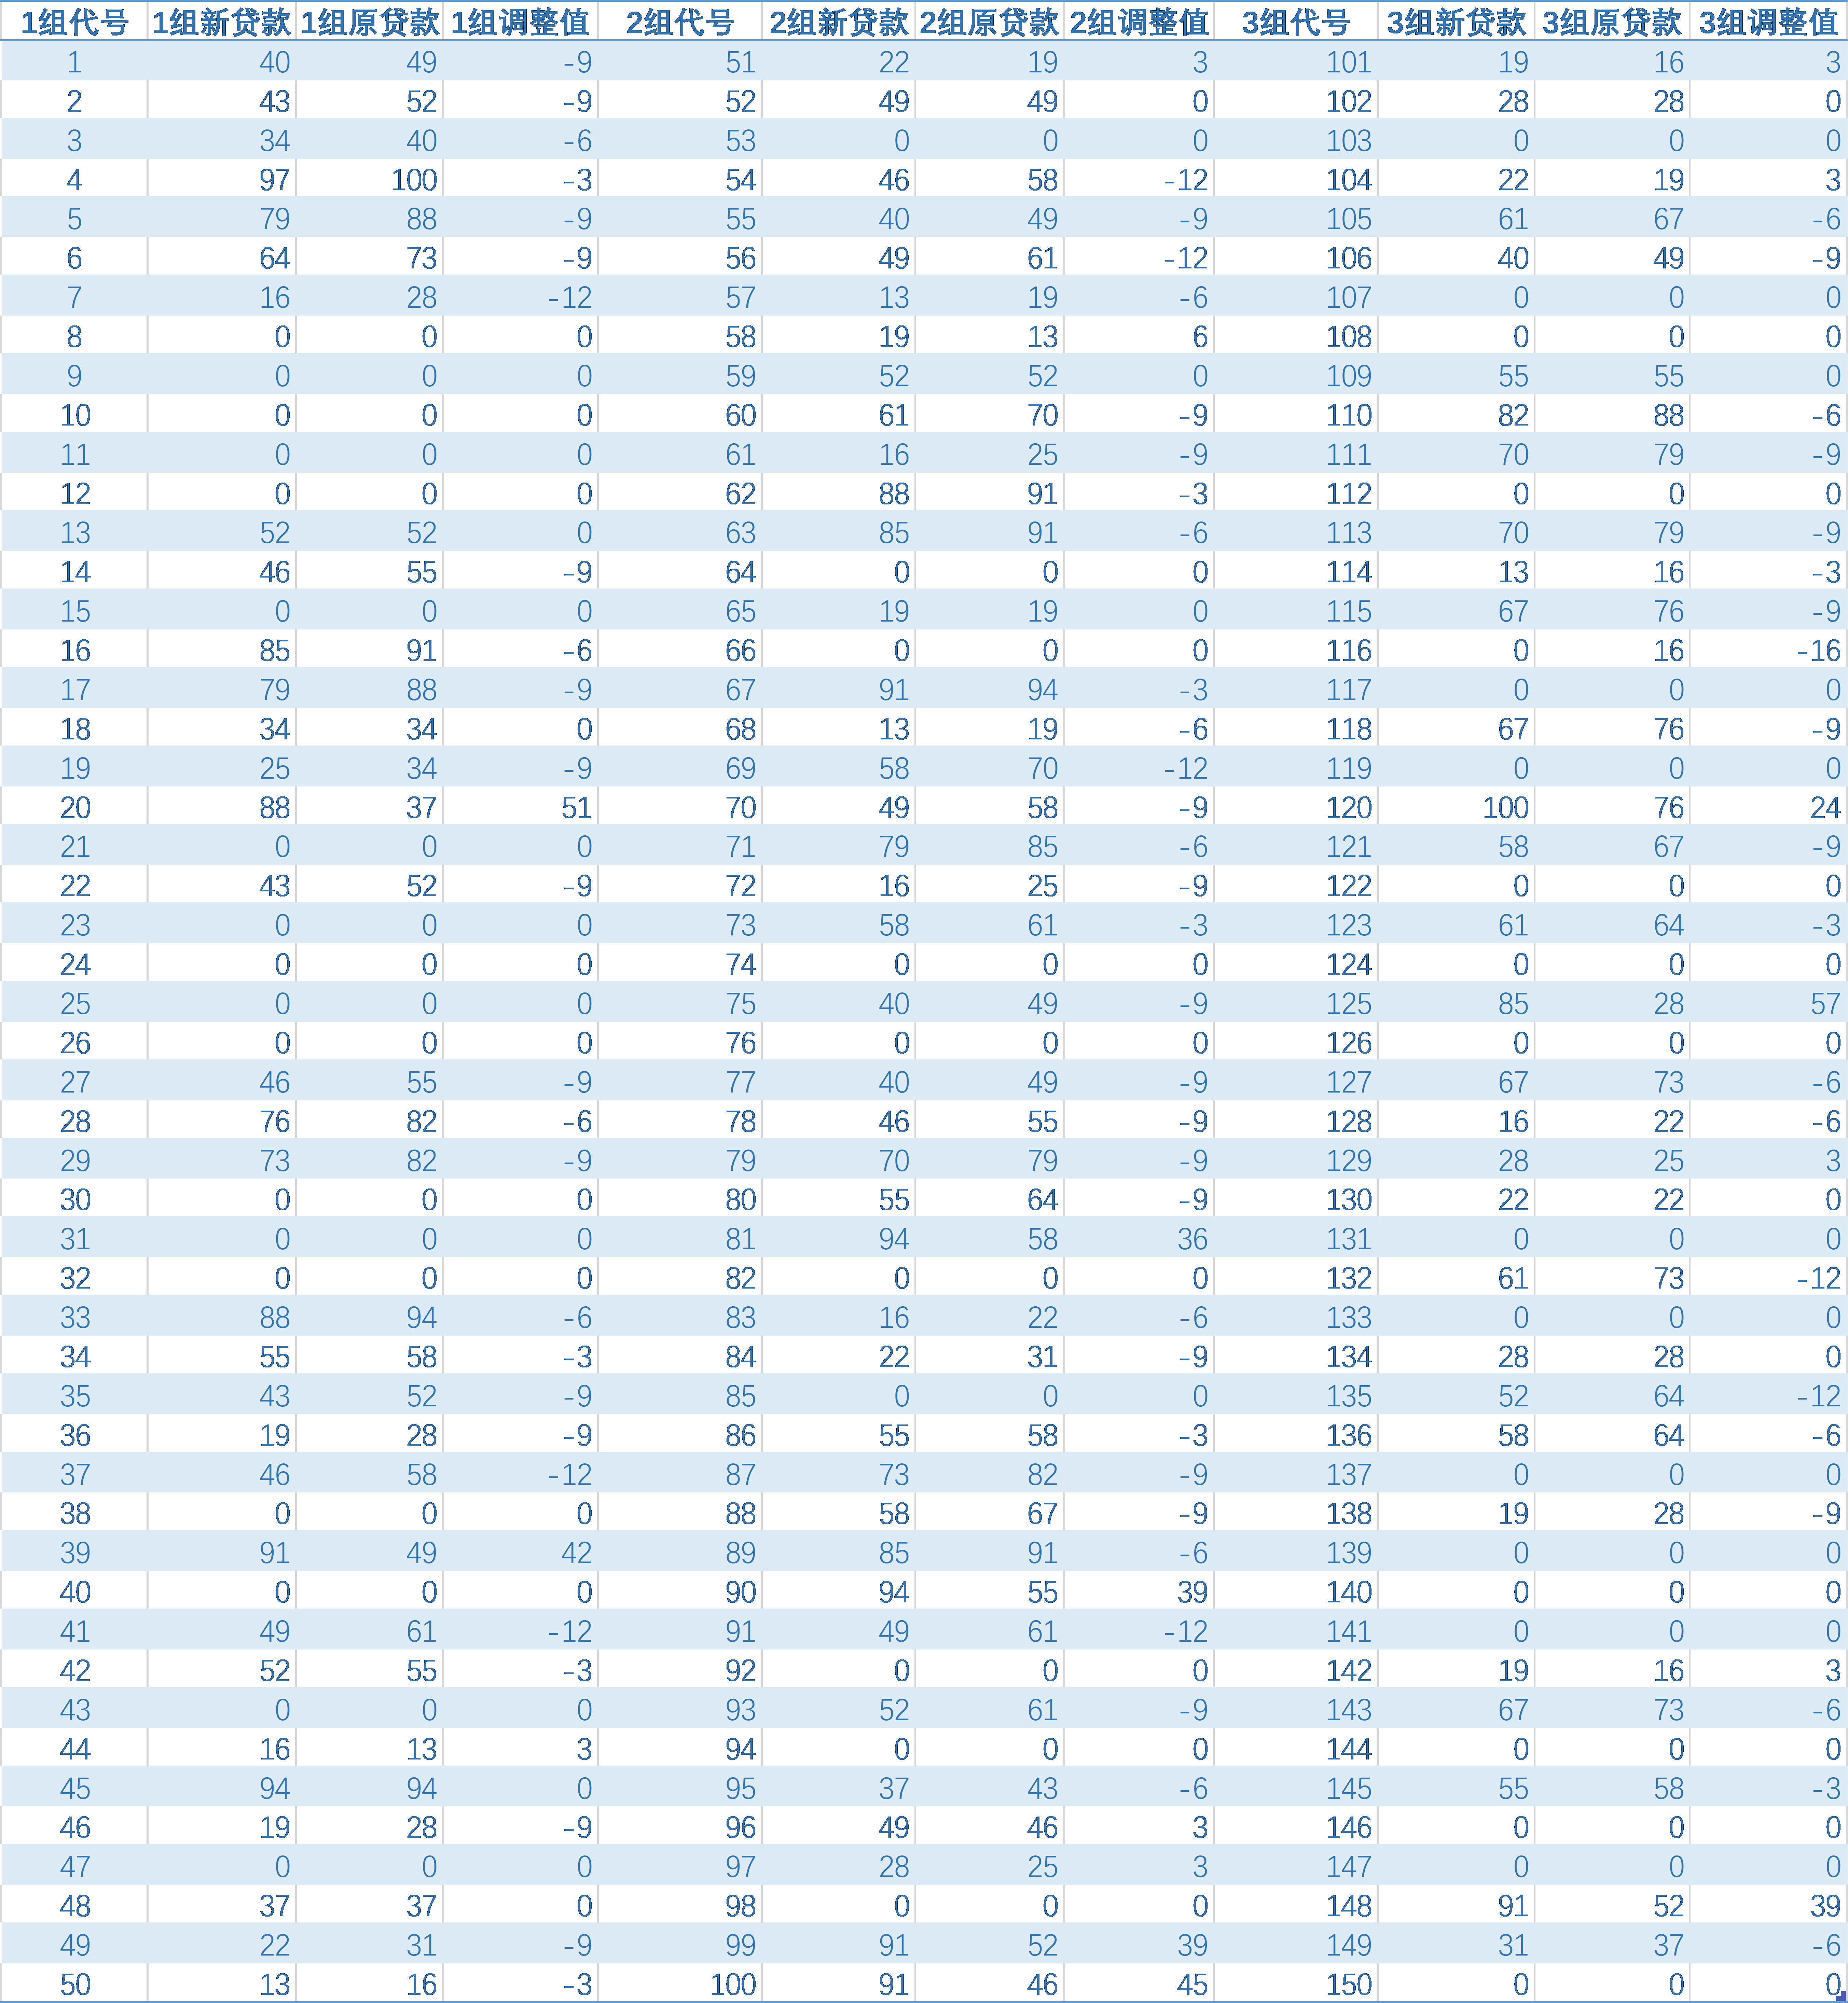
\includegraphics[width=1\linewidth]{figure/q3ResultTable}
	\caption{规划求解所得的信贷策略}
	\label{fig:q3ResultTable}
\end{figure}


\newpage

%分文件结束
\ifx\allfiles\undefined
\end{document}
\fi%问题三的建模与分析
%\ifx\allfiles\undefined
%生成目录超链接，使用UTF8字符集
\documentclass[12pt,UTF8]{ctexart}


\usepackage{mathtools}%花括号括起的公式
\usepackage{enumerate}%列表
\usepackage{graphicx}%表格
\usepackage[table]{xcolor}%彩色表格
\usepackage{booktabs}%调整表格行高


\renewcommand\tabcolsep{50pt}
\renewcommand\arraystretch{2}

%文本框
\usepackage{tcolorbox}
\tcbuselibrary{skins,vignette,raster,listings,listingsutf8,theorems, breakable,magazine,fitting}

%页面设置
\usepackage{geometry}%设置页面
\usepackage{setspace}%设置局部行距

\usepackage{ctex}
\usepackage{CJK}

%图像处理
\usepackage{graphicx}
\usepackage{float}%允许浮动
\usepackage{caption}%设置标题
\usepackage{graphicx, subfig}

%附录
\usepackage[toc,page]{appendix}

%导言区
\title{中小微企业的信贷决策}

%不要页眉
\pagestyle{plain}
\bibliographystyle{plain}

\geometry{a4paper}%将纸张设置为A4大小

%修改文档结构层次的名称
\usepackage{titlesec}%chapter1修改为一
\titleformat{\part}{\centering\Huge\bfseries}{\thepart}{1em}{}
\renewcommand\thepart{\chinese{part}}

%subsubsubsection的使用
%\usepackage{titlesec}
%\titleclass{\subsubsubsection}{straight}[\subsection]
%
%\newcounter{subsubsubsection}[subsubsection]
%\renewcommand\thesubsubsubsection{\thesubsubsection.\arabic{subsubsubsection}}
%\renewcommand\theparagraph{\thesubsubsubsection.\arabic{paragraph}}
%
%\titleformat{\subsubsubsection}
%{\normalfont\normalsize\bfseries}{\thesubsubsubsection}{1em}{}
%\titlespacing*{\subsubsubsection}
%{0pt}{3.25ex plus 1ex minus .2ex}{1.5ex plus .2ex}
%
%\makeatletter
%\renewcommand\paragraph{\@startsection{paragraph}{5}{\z@}%
%	{3.25ex \@plus1ex \@minus.2ex}%
%	{-1em}%
%	{\normalfont\normalsize\bfseries}}
%\renewcommand\subparagraph{\@startsection{subparagraph}{6}{\parindent}%
%	{3.25ex \@plus1ex \@minus .2ex}%
%	{-1em}%
%	{\normalfont\normalsize\bfseries}}
%\def\toclevel@subsubsubsection{4}
%\def\toclevel@paragraph{5}
%\def\toclevel@paragraph{6}
%\def\l@subsubsubsection{\@dottedtocline{4}{7em}{4em}}
%\def\l@paragraph{\@dottedtocline{5}{10em}{5em}}
%\def\l@subparagraph{\@dottedtocline{6}{14em}{6em}}
%\makeatother
%
%\setcounter{secnumdepth}{4}

\begin{document}
\else
\fi
%分文件开始


\subsection{问题四中旅游规划系统的开发}
\subsubsection{旅游规划系统的设计}
%先说一下一个用户界面应该有的特点，然后介绍一下我们的旅游规划系统的界面特点、结构特点等等

对一个旅游规划系统而言，其用户界面应具有以下几点主要特点：

首先是清楚性。用户界面设计的最终目的是为了使有不同需求的不同的人与系统通过沟通和功能来进行交互，因此一定的引导、解释是不可或缺的。

其次是简明性。用户界面应当为用户提供更加便捷、快速的渠道。

其三是高效率性。用户界面就像车辆，能准确的带用户去他想要到的地方。一个良好的界面能够让执行用户需求功能更快。

最后是吸引性。更具吸引力的界面不仅使得交互变得愉快，会让用户体验的满意度得以提升，还会让用户期待使用它。

~\\

本次我们所设计的张家界旅游规划系统正是遵从上述的四个主要特点来进行规划设计的。


\begin{figure}[H]
	\centering
	\includegraphics[width=1\linewidth]{figure/q4System}
	\caption{张家界旅行规划系统示意图}
	\label{fig:q4system}
\end{figure}


我们的用户界面由四个部分组合而成，分别为基本参数、必去地点、开支、结果面板。结构清晰，操作便捷，排列整齐有序。

在色彩方面，我们采用了以暖色调为主的风格设计，让使用的用户在视觉上不会感觉过于单一，从而影响使用的体验感与满意度。

在操作方面，我们采用键盘输入方式与按钮选择方式相结合，给用户提供更加快捷的方式，让他们可以在最短的时间内，找到满足要求的最合适的旅游线路以及对应的消费方案。在此系统中，还将根据近年来网上各景点的人气排名\cite{ref2}，推荐必去景点供用户选择，当然用户也可以手动输入想去的景点。用户可以根据系统引导，从左到右，从上到下依次进行操作，最终会在结果面板中得到答案。

在开支方面，我们设计的系统作出了进一步的细化供用户根据自身情况，进行相应的选择与输入，并将交通、食宿、门票各方面所需总额清楚的计算展现出来，让用户进一步了解各方面开支占比，从而极大的提高用户的使用效率，方便用户在接下来的旅游中进行详细的规划。


\subsubsection{旅游规划系统的使用}
%介绍一下这玩意怎么使用

首先，用户需在基本参数表中输入游玩的天数、人数、每日安排的游玩时间、总预算的基本信息，系统由此给出总游玩时间，从而进行下一步的安排.

接下来，用户可以在右侧表格必去地点中，采用手动输入或者按钮筛选输入的方式，选择在此次旅行安排中必去的地点，若有剩余的时间与预算，其余地点将由系统根据人气排名、最大限度利用时间与预算，进行合适的规划。

然后用户在开支面板中，首先挑选旅程所采用的交通方式，并依此自动计算所需费用。

其次，用户在食宿方面，可以自行输入每日食宿预算费用，同样系统也将自动计算总额。随后，根据用户选择的旅游景点，系统会依据每个景区的门票费用，自动计算出所需总额。

\begin{figure}[htbp]
	\centering
	\begin{minipage}[t]{0.49\textwidth}
		\centering
		\includegraphics[width=6cm]{figure/q4Input1}
	\end{minipage}
	\begin{minipage}[t]{0.49\textwidth}
		\centering
		\includegraphics[width=6cm]{figure/q4Input2}
	\end{minipage}
\end{figure}


\begin{figure}[H]
	\centering
	\includegraphics[width=0.7\linewidth]{figure/q4Input3}
	\label{fig:q4Input3}
\end{figure}


最后，用户会在结果面板中读取，此次张家界旅行的满意度总分、总开支、余额、总游玩时间与游玩景点数，并在右侧的旅游路线建议框中给出对应的具体游览景点顺序与路线。用户可由此做参考。

\begin{figure}[H]
	\centering
	\includegraphics[width=1\linewidth]{figure/q4Output}
	\caption{结果面板及旅游路线建议示意图}
	\label{fig:q4Output}
\end{figure}


\newpage


%分文件结束
\ifx\allfiles\undefined
\end{document}
\fi%问题四的建模与分析

\ifx\allfiles\undefined
%生成目录超链接，使用UTF8字符集
\documentclass[12pt,UTF8]{ctexart}


\usepackage{mathtools}%花括号括起的公式
\usepackage{enumerate}%列表
\usepackage{graphicx}%表格
\usepackage[table]{xcolor}%彩色表格
\usepackage{booktabs}%调整表格行高


\renewcommand\tabcolsep{50pt}
\renewcommand\arraystretch{2}

%文本框
\usepackage{tcolorbox}
\tcbuselibrary{skins,vignette,raster,listings,listingsutf8,theorems, breakable,magazine,fitting}

%页面设置
\usepackage{geometry}%设置页面
\usepackage{setspace}%设置局部行距

\usepackage{ctex}
\usepackage{CJK}

%图像处理
\usepackage{graphicx}
\usepackage{float}%允许浮动
\usepackage{caption}%设置标题
\usepackage{graphicx, subfig}

%附录
\usepackage[toc,page]{appendix}

%导言区
\title{中小微企业的信贷决策}

%不要页眉
\pagestyle{plain}
\bibliographystyle{plain}

\geometry{a4paper}%将纸张设置为A4大小

%修改文档结构层次的名称
\usepackage{titlesec}%chapter1修改为一
\titleformat{\part}{\centering\Huge\bfseries}{\thepart}{1em}{}
\renewcommand\thepart{\chinese{part}}

%subsubsubsection的使用
%\usepackage{titlesec}
%\titleclass{\subsubsubsection}{straight}[\subsection]
%
%\newcounter{subsubsubsection}[subsubsection]
%\renewcommand\thesubsubsubsection{\thesubsubsection.\arabic{subsubsubsection}}
%\renewcommand\theparagraph{\thesubsubsubsection.\arabic{paragraph}}
%
%\titleformat{\subsubsubsection}
%{\normalfont\normalsize\bfseries}{\thesubsubsubsection}{1em}{}
%\titlespacing*{\subsubsubsection}
%{0pt}{3.25ex plus 1ex minus .2ex}{1.5ex plus .2ex}
%
%\makeatletter
%\renewcommand\paragraph{\@startsection{paragraph}{5}{\z@}%
%	{3.25ex \@plus1ex \@minus.2ex}%
%	{-1em}%
%	{\normalfont\normalsize\bfseries}}
%\renewcommand\subparagraph{\@startsection{subparagraph}{6}{\parindent}%
%	{3.25ex \@plus1ex \@minus .2ex}%
%	{-1em}%
%	{\normalfont\normalsize\bfseries}}
%\def\toclevel@subsubsubsection{4}
%\def\toclevel@paragraph{5}
%\def\toclevel@paragraph{6}
%\def\l@subsubsubsection{\@dottedtocline{4}{7em}{4em}}
%\def\l@paragraph{\@dottedtocline{5}{10em}{5em}}
%\def\l@subparagraph{\@dottedtocline{6}{14em}{6em}}
%\makeatother
%
%\setcounter{secnumdepth}{4}

\begin{document}
\else
\fi
%分文件开始


\part{模型评价}

\noindent \textbf{模型的优点：}

\begin{enumerate}[(1)]
	%开始：优点
	\item 我们综合运用了Power BI、MATLAB等软件，使用层次分析法来量化分析附件1和附件2中企业的信贷风险，构建决策树模型来预测附件2中企业的信誉评级，并利用规划模型求解信贷策略。从模型评价上看，这些定量模型能够很好地反映实际情况，有效地解决了题目所提出的三个问题。
	\item 在问题三中，我们阅读了大量新闻报道以此了解疫情对企业的影响，以名称划分行业，以行业为单位确定影响程度，较好地反映了实际情况。

	%结束：优点	
\end{enumerate}

\noindent \textbf{模型的不足之处：}

\begin{enumerate}[(1)]
	%开始：不足之处	
	\item 本文根据企业信息、进项发票信息和销项发票信息来判定企业的信贷风险，但在现实中，与企业信贷风险关联的因素还有很多。
	\item 对于问题三，我们根据企业名称将企业分为13个行业，受4种不同程度的影响。但在现实中，疫情对企业的影响要精细得多。

	%结束：不足之处	
\end{enumerate}



%分文件结束
\ifx\allfiles\undefined
\end{document}
\fi%模型评价

%结尾部分
\ifx\allfiles\undefined
%生成目录超链接，使用UTF8字符集
\documentclass[12pt,UTF8]{ctexart}


\usepackage{mathtools}%花括号括起的公式
\usepackage{enumerate}%列表
\usepackage{graphicx}%表格
\usepackage[table]{xcolor}%彩色表格
\usepackage{booktabs}%调整表格行高


\renewcommand\tabcolsep{50pt}
\renewcommand\arraystretch{2}

%文本框
\usepackage{tcolorbox}
\tcbuselibrary{skins,vignette,raster,listings,listingsutf8,theorems, breakable,magazine,fitting}

%页面设置
\usepackage{geometry}%设置页面
\usepackage{setspace}%设置局部行距

\usepackage{ctex}
\usepackage{CJK}

%图像处理
\usepackage{graphicx}
\usepackage{float}%允许浮动
\usepackage{caption}%设置标题
\usepackage{graphicx, subfig}

%附录
\usepackage[toc,page]{appendix}

%导言区
\title{中小微企业的信贷决策}

%不要页眉
\pagestyle{plain}
\bibliographystyle{plain}

\geometry{a4paper}%将纸张设置为A4大小

%修改文档结构层次的名称
\usepackage{titlesec}%chapter1修改为一
\titleformat{\part}{\centering\Huge\bfseries}{\thepart}{1em}{}
\renewcommand\thepart{\chinese{part}}

%subsubsubsection的使用
%\usepackage{titlesec}
%\titleclass{\subsubsubsection}{straight}[\subsection]
%
%\newcounter{subsubsubsection}[subsubsection]
%\renewcommand\thesubsubsubsection{\thesubsubsection.\arabic{subsubsubsection}}
%\renewcommand\theparagraph{\thesubsubsubsection.\arabic{paragraph}}
%
%\titleformat{\subsubsubsection}
%{\normalfont\normalsize\bfseries}{\thesubsubsubsection}{1em}{}
%\titlespacing*{\subsubsubsection}
%{0pt}{3.25ex plus 1ex minus .2ex}{1.5ex plus .2ex}
%
%\makeatletter
%\renewcommand\paragraph{\@startsection{paragraph}{5}{\z@}%
%	{3.25ex \@plus1ex \@minus.2ex}%
%	{-1em}%
%	{\normalfont\normalsize\bfseries}}
%\renewcommand\subparagraph{\@startsection{subparagraph}{6}{\parindent}%
%	{3.25ex \@plus1ex \@minus .2ex}%
%	{-1em}%
%	{\normalfont\normalsize\bfseries}}
%\def\toclevel@subsubsubsection{4}
%\def\toclevel@paragraph{5}
%\def\toclevel@paragraph{6}
%\def\l@subsubsubsection{\@dottedtocline{4}{7em}{4em}}
%\def\l@paragraph{\@dottedtocline{5}{10em}{5em}}
%\def\l@subparagraph{\@dottedtocline{6}{14em}{6em}}
%\makeatother
%
%\setcounter{secnumdepth}{4}

\begin{document}
\else
\fi
%分文件开始


%参考文献
\begin{thebibliography}{99}
	%在没有原样抄写的情况下，网站中的“#”、“_”改成“\#”、“\_”，前面加一个反斜杠
	%现已有原样抄写的环境下，可以直接将链接放入

	%开始：参考文献
	\bibitem{ref1} \verb|司守奎、孙兆亮，《数学建模算法与应用》（第二版）[M]，国防工业出版社，2016。|
	\bibitem{ref2} \verb|姜启源，《数学模型》[M]，高等教育出版社，1993。|
	%\bibitem{ref3} \verb|曹明，预测评价指标RMSE、MSE、MAE、MAPE、SMAPE，https://www.cnblogs.com/think90/articles/11786016.html，2020年9月12日。|
	%\bibitem{ref4} \verb|easyAI，决策树 – Decision tree，https://easyai.tech/ai-definition/decision-tree/，2020年09月12日。|
	\bibitem{ref3} \verb|新浪财经，新冠肺炎疫情对若干行业的影响分析[OL]，https://finance.sina.com.cn/review/jcgc/2020-02-08/doc-iimxyqvz1258307.shtml，2020年9月12日。|

	%\bibitem{ref4} \verb||
	%\bibitem{ref5} \verb||
	%\bibitem{ref6} \verb||

	%结束：参考文献
\end{thebibliography}
\addcontentsline{toc}{section}{参考文献}%将“参考文献”字样加入目录中


\newpage


%分文件结束
\ifx\allfiles\undefined
\end{document}
\fi%参考文献
\ifx\allfiles\undefined
%生成目录超链接，使用UTF8字符集
\documentclass[12pt,UTF8]{ctexart}


\usepackage{mathtools}%花括号括起的公式
\usepackage{enumerate}%列表
\usepackage{graphicx}%表格
\usepackage[table]{xcolor}%彩色表格
\usepackage{booktabs}%调整表格行高


\renewcommand\tabcolsep{50pt}
\renewcommand\arraystretch{2}

%文本框
\usepackage{tcolorbox}
\tcbuselibrary{skins,vignette,raster,listings,listingsutf8,theorems, breakable,magazine,fitting}

%页面设置
\usepackage{geometry}%设置页面
\usepackage{setspace}%设置局部行距

\usepackage{ctex}
\usepackage{CJK}

%图像处理
\usepackage{graphicx}
\usepackage{float}%允许浮动
\usepackage{caption}%设置标题
\usepackage{graphicx, subfig}

%附录
\usepackage[toc,page]{appendix}

%导言区
\title{中小微企业的信贷决策}

%不要页眉
\pagestyle{plain}
\bibliographystyle{plain}

\geometry{a4paper}%将纸张设置为A4大小

%修改文档结构层次的名称
\usepackage{titlesec}%chapter1修改为一
\titleformat{\part}{\centering\Huge\bfseries}{\thepart}{1em}{}
\renewcommand\thepart{\chinese{part}}

%subsubsubsection的使用
%\usepackage{titlesec}
%\titleclass{\subsubsubsection}{straight}[\subsection]
%
%\newcounter{subsubsubsection}[subsubsection]
%\renewcommand\thesubsubsubsection{\thesubsubsection.\arabic{subsubsubsection}}
%\renewcommand\theparagraph{\thesubsubsubsection.\arabic{paragraph}}
%
%\titleformat{\subsubsubsection}
%{\normalfont\normalsize\bfseries}{\thesubsubsubsection}{1em}{}
%\titlespacing*{\subsubsubsection}
%{0pt}{3.25ex plus 1ex minus .2ex}{1.5ex plus .2ex}
%
%\makeatletter
%\renewcommand\paragraph{\@startsection{paragraph}{5}{\z@}%
%	{3.25ex \@plus1ex \@minus.2ex}%
%	{-1em}%
%	{\normalfont\normalsize\bfseries}}
%\renewcommand\subparagraph{\@startsection{subparagraph}{6}{\parindent}%
%	{3.25ex \@plus1ex \@minus .2ex}%
%	{-1em}%
%	{\normalfont\normalsize\bfseries}}
%\def\toclevel@subsubsubsection{4}
%\def\toclevel@paragraph{5}
%\def\toclevel@paragraph{6}
%\def\l@subsubsubsection{\@dottedtocline{4}{7em}{4em}}
%\def\l@paragraph{\@dottedtocline{5}{10em}{5em}}
%\def\l@subparagraph{\@dottedtocline{6}{14em}{6em}}
%\makeatother
%
%\setcounter{secnumdepth}{4}

\begin{document}
\else
\fi
%分文件开始

\appendix
\renewcommand{\appendixpagename}{附录}
\renewcommand{\appendixtocname}{附录}
%附录开始
\begin{appendices}

\noindent \textbf{{\large 支撑材料清单：}}
\begin{enumerate}[(1)]
	\item 问题1多元线性规划求解代码：Q1LP.mlx 
	\item 问题2多元线性规划求解源代码：Q2LP.mlx 
	\item 问题3多元线性规划求解源代码：Q3LP.mlx 
	\item 问题1、2层次分析法源代码：Q2Work.mlx 
	\item 问题3层次分析法源代码：Q3Work.mlx
	\item 多元线性回归源数据：附件1分档.xIsx
	\item 多元线性回归源数据：附件2分档.xIsx
	\item 多元线性回归源数据：问题3附件2分档.xlsx
	\item 规划求解结果.xlsx
	\item 决策树训练结果.pdf
	\item PowerBI数据处理.pbix
	\item 问题1数据处理.xIsx
	\item 问题2数据处理.xIsx
	\item 问题3数据处理.xIsx
\end{enumerate}

	\section{问题一中层次分析法的MATLAB实现}

	首先编写实现单层次结构的层次分析法的\verb|AHP(A)|函数
	\begin{tcolorbox}[breakable]
		\begin{verbatim}
		function [W, Lmax, CI, CR] = AHP(A)
		% 实现单层次结构的层次分析法
		% 输入: A为成对比较矩阵
		% 输出: W为权重向量, Lmax为最大特征值, CI为一致性指标, CR为一致性比率
		
		[V,D] = eig(A);
		[Lmax,ind] = max(diag(D));       % 求最大特征值及其位置
		W = V(:,ind) / sum(V(:,ind));    % 最大特征值对应的特征向量做标准化
		Lmax = mean((A * W) ./ W);       % 计算最大特征值
		n = size(A, 1);                  % 矩阵行数
		CI = (Lmax - n) / (n - 1);       % 计算一致性指标
		% Saaty随机一致性指标值
		RI = [0 0 0.58 0.90 1.12 1.24 1.32 1.41 1.45 1.49 1.51]; 
		CR = CI / RI(n);                 % 计算一致性比率
	 \end{verbatim}
	\end{tcolorbox}

	按照如下代码构建目标层与准则层之间的成对比较矩阵，并调用\verb|AHP(A)|，即可得到组合权向量：

	\begin{tcolorbox}[breakable]
		\begin{verbatim}
		%目标层与准则层之间的成对比较矩阵
		A =
		[1  8  3  5  6  1; 
			1/8  1  1/7  1/5  1/4  1/8;
			 1/3  7  1  3  2  1/3;
			 1/5  5  1/3  1  1/3  1/5;
			 1/6  4  1/2  3  1  1/4;
			 	1  8  3  5  4  1;];
		[W, Lmax, CI, CR] = AHP(A)
	\end{verbatim}
	\end{tcolorbox}


	\section{问题一中规划模型的MALTAB实现}
	\begin{tcolorbox}[breakable]
		\begin{verbatim}
%Part1:导入数据
%此处xlsread函数的参数含义:路径，读取第一个工作表，读取单元格范围
%年利率
AnnualInterestRate = xlsread("D:\OneDrive\GitHub\CUMCM2020材料包\附件1分档.xlsx",1,'F11:F133');
%保有率
RetentionRate = xlsread("D:\OneDrive\GitHub\CUMCM2020材料包\附件1分档.xlsx",1,'G11:G133');
%最大贷款额度
MaxLoanLimit = xlsread("D:\OneDrive\GitHub\CUMCM2020材料包\附件1分档.xlsx",1,'H11:H133');



%Part2:运算台
%xi的权重向量ki=该企业的保有率*年利率*1年
k=AnnualInterestRate'.*RetentionRate'.*1;
%企业数
n=123;
%银行信贷总额，单位万元
total=3050:100:5000;
num=size(total,2);

%Part3:规划求解
%目标函数中，xi的权重向量f
%目标函数应标准化求解最小值
f=-k;

%不等式约束条件A,Ax<=b，inequality constraint
A=[eye(n) ;ones(1,n)];

%等式约束条件aeqx=beq，equality constraint
aeq=zeros(1,n);
beq=0;

%xi的上下界，bound constraint
lb=zeros(n,1);
ub=100*ones(n,1);



%Part4:结果台
%预分配内存
income=zeros(1,num);
test=zeros(n,num);

%构建循环
for i = 1:1:num
b=[MaxLoanLimit;total(i)];

%各家企业实际贷款额度
x=linprog(f,A,b,aeq,beq,lb,ub);

%银行收入
%目标函数反向标准化，求解最大值
income(i)=sum(-f.*x,'all');

test(:,i)=x;
end

plot(total,income)
test
	\end{verbatim}
	\end{tcolorbox}



	\section{问题二中决策树模型的工程参数}
	\begin{center}
		\begin{table}[H]  %table 里面也可以嵌套tabular,只有tabular是不能加标题的
			\centering
			\resizebox{300pt}{200pt}{
				\begin{tabular}{cc}
					\hline
					参数名                           & 参数值 \\
					\hline
					数据切分                         & 0.75   \\
					数据洗牌                         & 是     \\
					交叉验证                         & 否     \\
					随机种子                         & 0      \\
					分裂准则                         & mse    \\
					树的最大深度                     & None   \\
					分裂节点时的策略                 & best   \\
					分裂一个内部节点所需最少样本数   & 2      \\
					每个叶子节点所需最少样本数       & 2      \\
					叶子节点中样本的最小权重         & 0      \\
					搜寻最佳划分的时候考虑的特征数量 & None   \\
					叶子节点的最大数量               & None   \\
					信息墒或者基尼系数不纯度的阀值   & 0      \\
					\hline
				\end{tabular}}
		\end{table}
	\end{center}

	\section{问题二中规划模型的MATLAB实现}
	\begin{tcolorbox}[breakable]
		\begin{verbatim}
		%Part1:导入数据
		%此处xlsread函数的参数含义:路径，读取第一个工作表，读取单元格范围
		%年利率
		AnnualInterestRate = xlsread("D:\OneDrive\GitHub\CUMCM2020材料包\附件2分档.xlsx",1,'F11:F312');
		%保有率
		RetentionRate = xlsread("D:\OneDrive\GitHub\CUMCM2020材料包\附件2分档.xlsx",1,'G11:G312');
		%最大贷款额度
		MaxLoanLimit = xlsread("D:\OneDrive\GitHub\CUMCM2020材料包\附件2分档.xlsx",1,'H11:H312');
		
		
		
		%Part2:运算台
		%xi的权重向量ki=该企业的保有率*年利率*1年
		k=AnnualInterestRate'.*RetentionRate'.*1;
		%企业数
		n=302;
		%银行信贷总额，单位万元
		total=10000;
		
		
		
		%Part3:规划求解
		%目标函数中，xi的权重向量f
		%目标函数应标准化求解最小值
		f=-k
		
		%不等式约束条件Ax<=b，inequality constraint
		A=[eye(n) ;ones(1,n)];
		b=[MaxLoanLimit;total];
		
		%等式约束条件aeqx=beq，equality constraint
		aeq=zeros(1,n);
		beq=0;
		
		%xi的上下界，bound constraint
		lb=zeros(n,1);
		ub=100*ones(n,1);
		
		
		
		%Part4:结果台
		%各家企业实际贷款额度
		x=linprog(f,A,b,aeq,beq,lb,ub)
		
		%银行收入，单位万元
		%目标函数反向标准化，求解最大值
		income=sum(-f.*x,'all')
	\end{verbatim}
	\end{tcolorbox}


	\section{问题三中层次分析法的MATLAB实现}
	\begin{tcolorbox}[breakable]
		\begin{verbatim}
A = 
[1  5  7  9  3;
1/5  1  3  1/5  1;
1/7  1/3  1  5  1/5;
1/9  1/5  1/5  1  1/7;
1/3  1  5  7  1;];
[W, Lmax, CI, CR] = AHP(A)
	\end{verbatim}
	\end{tcolorbox}

	\section{问题三中规划模型的MATLAB实现}
	\begin{tcolorbox}[breakable]
		\begin{verbatim}
%Part1:导入数据
%此处xlsread函数的参数含义:路径，读取第一个工作表，读取单元格范围
%年利率
AnnualInterestRate = xlsread("D:\OneDrive\GitHub\CUMCM2020材料包\问题3附件2分档.xlsx",1,'F11:F312');
%保有率
RetentionRate = xlsread("D:\OneDrive\GitHub\CUMCM2020材料包\问题3附件2分档.xlsx",1,'G11:G312');
%最大贷款额度
MaxLoanLimit = xlsread("D:\OneDrive\GitHub\CUMCM2020材料包\问题3附件2分档.xlsx",1,'H11:H312');
%问题2求解结果
Q2Result = xlsread("D:\OneDrive\GitHub\CUMCM2020材料包\规划求解结果.xlsx",1,'S2:S303');



%Part2:运算台
%xi的权重向量ki=该企业的保有率*年利率*1年
k=AnnualInterestRate'.*RetentionRate'.*1;
%企业数
n=302;
%银行信贷总额，单位万元
total=10000;



%Part3:规划求解
%目标函数中，xi的权重向量f
%目标函数应标准化求解最小值
f=-k

%不等式约束条件Ax<=b，inequality constraint
A=[eye(n) ;ones(1,n)];
b=[MaxLoanLimit;total];

%等式约束条件aeqx=beq，equality constraint
aeq=zeros(1,n);
beq=0;

%xi的上下界，bound constraint
lb=zeros(n,1);
ub=100*ones(n,1);



%Part4:结果台
%各家企业实际贷款额度
x=linprog(f,A,b,aeq,beq,lb,ub)

%银行收入
%目标函数反向标准化，求解最大值
income=sum(-f.*x,'all')

Delta=x-Q2Result
	\end{verbatim}
	\end{tcolorbox}


	%附录结束
\end{appendices}


%分文件结束
\ifx\allfiles\undefined
\end{document}
\fi%代码或数据


%Part2:figure文件夹
%存放LaTeX中需要使用的图片


}
\end{document}